%\documentclass[10pt]{article}
\documentclass[10pt]{book}

\usepackage[draft]{fixme}

\usepackage{listings}

\usepackage{html}
\usepackage{color}

\usepackage{multicol}
\usepackage{multirow}

\usepackage{graphicx}
\usepackage{alltt}

\newcommand{\hlstd}[1]{\textcolor[rgb]{0,0,0}{#1}}
\newcommand{\hlkey}[1]{\textcolor[rgb]{0,0,0}{\bf{#1}}}
\newcommand{\hlnum}[1]{\textcolor[rgb]{0.16,0.16,1}{#1}}
\newcommand{\hltyp}[1]{\textcolor[rgb]{0.51,0,0}{#1}}
\newcommand{\hlesc}[1]{\textcolor[rgb]{1,0,1}{#1}}
\newcommand{\hlstr}[1]{\textcolor[rgb]{1,0,0}{#1}}
\newcommand{\hldstr}[1]{\textcolor[rgb]{0.51,0.51,0}{#1}}
\newcommand{\hlcom}[1]{\textcolor[rgb]{0.51,0.51,0.51}{\it{#1}}}
\newcommand{\hldir}[1]{\textcolor[rgb]{0,0.51,0}{#1}}
\newcommand{\hlsym}[1]{\textcolor[rgb]{0,0,0}{#1}}
\newcommand{\hlline}[1]{\textcolor[rgb]{0.33,0.33,0.33}{#1}}

\newcommand{\mySmallFontSize}{\scriptsize}
\newcommand{\mySmallestFontSize}{\tiny}

\newcommand{\codeFontSize}{\scriptsize}
\newcommand{\code}[1]{{\scriptsize #1}}

% Software version number
\newcommand{\VersionNumber}{0.9.5a}

\newcommand{\ExampleDirectory}{../../../../../../projects/compass/tests}

% Latex trick to allow us to comment out large sections of documentation
\newcommand{\commentout}[1]{}

% change the title of the Fixme List
\renewcommand{\listfixmename}{Things to Fix in Documentation of Compass}

\newcommand{\comm}[2]{\bigskip
                      \begin{tabular}{|p{11cm}|}\hline
                      \multicolumn{1}{|c|}{{\bf Comment by #1}}\\ \hline
                      #2\\ \hline
                      \end{tabular}
                      \bigskip
                     }

\def\verbatimfile#1{\begingroup
                    \@verbatim \frenchspacing \@vobeyspaces
                    \input#1 \endgroup
}



\newcounter{lineno}

% Taken from verbatimfiles.sty on web
\makeatletter %JCL

\def\verbatimlisting#1{\setcounter{lineno}{0}%
    \begingroup \@verbatim \frenchspacing \@vobeyspaces \parindent=20pt
    \everypar{\stepcounter{lineno}\llap{\thelineno\ \ }}\input#1
    \endgroup
}

\makeatother %JCL

% \endinput


%\addtolength{\oddsidemargin}{-0.5in}
%\addtolength{\evensidemargin}{-0.5in}
\addtolength{\textheight}{0.5in}
%\addtolength{\textwidth}{0.5in}
%\addtolength{\textwidth}{1.0in}
%\addtolength{\topmargin}{-0.5in}
%\addtolength{\textheight}{1.5in}

% \pagenumbering{roman}
% \pagestyle{empty}
% \setcounter{page}{0}
% \thispagestyle{empty}

\sloppy

%---------------------------------------------------------------------
% Begin Document
%---------------------------------------------------------------------

\begin{document}
%\bibliographystyle{plain}
%

% This draft mode eliminates the figures (leaves boxes for where they would be)
%\psdraft

\title{ {\bf \textcolor{red}{         Compass User Manual: \\ 
                                A Tool for Source Code Checking \\
                                        (A ROSE Tool)} \\
                               \textcolor{blue}{Draft User Manual} \\
                               \textcolor{green}{(Associated with ROSE Version 0.9.5a)} } }

\author{ {\bf ROSE Team} \\
         Lawrence Livermore National Laboratory \\ 
         Livermore, CA  94550 \\
         925-423-2668 (office)  925-422-6278 (fax) \\
         {dquinlan}@llnl.gov \\
         Project Web Page: http://www.rosecompiler.org \\
         %Project Web Page: www.llnl.gov/casc/rose \\
         UCRL Number for ROSE User Manual: UCRL-SM-210137-DRAFT \\
         UCRL Number for ROSE Tutorial: UCRL-SM-210032-DRAFT \\
         UCRL Number for ROSE Source Code: UCRL-CODE-155962 \\ \\
         %\htmladdnormallink{ROSE User Manual (pdf)}{../ROSE_UserManual/ROSE-0.9.5a-UserManual.pdf} \\
         \htmladdnormallink{ROSE User Manual
         (pdf)}{http://www.rosecompiler.org/ROSE_UserManual/ROSE-0.9.5a-UserManual.pdf} \\
         \htmladdnormallink{ROSE Tutorial
         (pdf)}{http://www.rosecompiler.org/ROSE_Tutorial/ROSE-0.9.5a-Tutorial.pdf} \\
         \htmladdnormallink{ROSE HTML Reference (html
         only)}{http://www.rosecompiler.org/ROSE_HTML_Reference/index.html}
       }

% \textcolor{blue}{Compiler infrastructure for tools is a bit} \\
% \textcolor{blue}{like a cannon, sometime more than you really need,} \\ 
% \textcolor{blue}{but often all that it takes to solve the problem} \\

% This doesn't seem to work.  References to this label are not resolved.
\label{Compass:postscriptVersionOfUserManual}

\begin{htmlonly}
   \centering \includegraphics[width=3in]{../compass_rose.gif}
\end{htmlonly}

\maketitle

\begin{htmlonly}
   \centering \includegraphics[width=5in]{../compass_rose.gif}
\end{htmlonly}


%\begin{center}
%\today
%\end{center}

%\newpage
%\input{Copyright}
%\newpage

\newpage

%
\chapter*{Preface}

%  Purpose:
% \begin{itemize}
%    \item a. Welcome 
%    \item b. Program features
%    \item c. Program benefits
% \end{itemize}
% \begin{center}
% *********************  \newline
% \end{center}
% \vspace{0.25in}

   Welcome to the ROSE Compiler Framework Project.  The purpose of this project is to 
provide a mechanism for construction of specialized source-to-source translators 
(sometime referred to less precisely as {\em preprocessors}).  ROSE provides 
simple programmable mechanisms to read and rewrite the abstract syntax trees generated 
by separate compiler front-ends.  ROSE includes the Edison Design Group (EDG) 
front-end (in binary form within public
distributions), and is internally based upon SAGE III, thus ROSE is presently specific 
to the generation of C and C++ source-to-source based compilers ({\em translators}, 
more precisely).  Other language front-ends may be appropriate to add to ROSE in 
the future (current work with Rice University is focused on the addition of Open64's
front-end to ROSE as part of support for FORTRAN 90).

   ROSE makes it easy to build complex source-to-source translator
(preprocessor) tools, and thus supports research work in many areas:
\begin{itemize}
   \item Performance Optimization
   \item General Program Transformations
   \item Instrumentation
   \item Program Analysis
   \item Interface Generation
   \item Automated Check-pointing
   \item Software Security Analysis
   \item Software Verification
   \item Automated Unit Test Generation
   \item ... and much more ...
\end{itemize}


%\input{Forward}

% This fixes the really long table of contents problem
\setcounter{tocdepth}{1}

\tableofcontents
%\listoffigures
%\listoftables
\newpage
%

\section*{Acknowledgments}
%\chapter*{Acknowledgments}

   This tool is the product of the entire ROSE team. Compass
depends upon the ROSE open compiler infrastructure and is a
simple application of mechanisms in ROSE which have been 
developed over several years and contributed to by a large 
number of people.

This currently includes:

\begin{itemize}
   \item Staff: Dan Quinlan
   \item Post docs: Thomas Panas, Chunhua Liao, and Jeremiah Willcock
   \item Ex Post doc: Richard Vuduc 
   \item Students: \\
         Gergo Barany, Michael Byrd, Valentin David, Han Kim, Robert Preissl,
         Andreas Saebjornsen, Jacob Sorensen, Ramakrishna Upadrasta, 
         Jeremiah Willcock, Gary Yuan
   \item Internal LLNL Contributors: Greg White
   \item External Collaborators: \\ 
         We want to thank CERT, who has been particularly helpful and supportive both
         with the development of checkers for their Secure Coding Rules and with 
         numerous suggestions.
\end{itemize}



\newpage

\chapter{Introduction}

\section{Overview}

\label{introduction::overview}

   Compass is a tool for the checking of source code.  It is
based on the ROSE compiler infrastructure and demonstrates to
use of ROSE to build lots of simple pattern detectors for analysis
of C, C++, and Fortran source code.

   The purpose of this work is several fold:
\begin{itemize}
   \item Provide a concrete tool to support interactions with lab customers.
   \item Provide a home for the security analysis specific detectors being built within
         external research projects.
   \item Provide an external tool for general analysis of software.
   \item Provide a tool to support improvements to the ROSE source code base.
   \item Define an infrastructure for an evolving and easily tailored program analysis tool.
   \item Provide a simple motivation for expanded use of ROSE by external users.
         Development, testing, and evaluation of ROSE infrastructure is best facilitated 
         through its expanded use by others and this provides a specific and attractive
         tool that can provide feedback to users about their own code projects.  Even
         though optimization research is our focus, this gets our supporting
         infrastructure for optimization research out and into use by others in the form
         of an extensible tool.
\end{itemize}

   Note that as the collection of detectors grows we will periodically reorganize the 
collection.  At some point soon we will build a hierarchy to organize the evolving
collection.

%\subsection{A basis for other source analysis tools}
\paragraph{A basis for other source analysis tools}
   Input and output to ROSE is organized so that any number of source could be used.
So although we provide a compiler interface (for simplicity), we will also provide a 
GUI interface as an alternative interface to demonstrate that the detectors are orthogonal
to there use in alternative tools.  Alternative tool interfaces should be possible 
and will further demonstrate the independence of the input and output mechanisms to
the designs and implementation of the core detectors.

\paragraph{Add Your Own Detector}

    Detectors written in Compass make direct use of ROSE and are 
designed to be copied and extended by users to develop their own 
detectors. We welcome the contribution of these detectors back to 
the ROSE team for inclusion into future releases of Compass;
full credit for all work will be provide to all authors.
Compass is an open source project using ROSE, an open source
compiler infrastructure.

    Each of the detectors are examples of how to
add your own detector to {\bf Compass}.  If you
build a detector that you would like to have be 
distributed with {\bf Compass}, please send it to
us and we will add your as an external contributor.

  Guidelines for contributions:
\begin{itemize}
   \item Use any Compass detector and an example.
   \item provide the documentation about your detector.
   \item Use any features in ROSE to support your detector; AST, Control Flow graph,
    System dependence Graph, Call Graph, Class Hierarchy Graph, etc.
   \item Your detector should have {\bf NO} side-effects on the AST.
\end{itemize}






\chapter{Design}


\section{Use Cases}

\label{design::UseCase}

Figure~\ref{Compass_usecase} shows the use cases of \emph{Compass}.
Compass as a tool is used to analyze source code. The analysis is triggered by the user who
selects which detectors to execute. The user also specifies the source code to be checked.
Results of the analysis are presented to that user.

\begin{figure}[th]
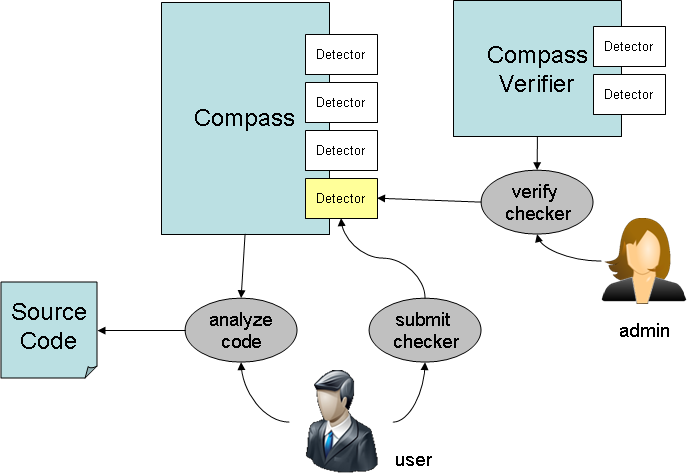
\includegraphics[width=4.5in]{compass_pic.png}
\caption{Compass Use Case}
\label{Compass_usecase}
\end{figure}

Furthermore, a user may contribute with his own detectors that he can add to Compass. Since 
external users may contribute detectors automatically via scripts, a verification of the 
validity and safety of these detectors is necessary. We provide a \emph{Compass Verifier}
that helps to check that all detectors are safe. Currently, the verifier is run by
a administrative person but may run automatically in the future.



\section{Design}

\begin{figure}[thb]
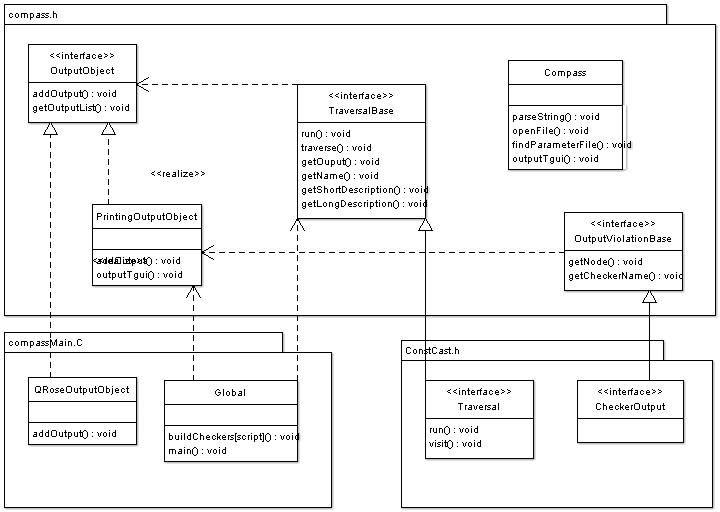
\includegraphics[width=6.0in]{compassdesign.png}
\caption{Compass Design}
\label{CompassDesign}
\end{figure}

Compass is designed to be easy to extend. Any user may write a detector and add it to Compass. Figure~\ref{CompassDesign}
illustrates the UML design decisions behind Compass.


Most of the functionality of Compass is in abstract classes hidden in the Compass namespace within compass.h - a file within
the compassSupport directory. All detectors, such as ConstCast illustrated in the figure, utilize the abstract classes
to traverse a program with all its nodes and to output violations found in that code according to the local algorithm.

CompassMain is the main executable that initially calls ROSE to parse a program. Then \emph{buildCheckers} is called to
load all detectors that are specified within a configuration file. The configuration file allows users to turn on and off
specific detectors for their run-time analyses. However, the configuration file only permits detectors to be loaded that 
were part of Compass at compile-time.

The main interface file compass.h contains the abstract classes \emph{TraversalBase} and 
\emph{OutputObject}. TraversalBase is the interface to ROSE, allowing a detector to traverse the ROSE AST (program) and hence
perform analysis on that AST. OutputObject aids to output defects found by a specific detector. More functionality to handle
e.g. file input and parameters provided to Compass, is provided within the Compass namespace.


\section{Compass Verifier}

\subsection{Threats} 

Compass must be safe, so that analyses and their results can be trusted. 
The main threats to the validity of Compass are:

\begin{itemize}
\item \emph{Malicious User}. A malicious user is an external user of Compass contributing a detector that performs malicious behaviour.  
\item \emph{Malicious Detector}. Compass is extensible and new detectos can be added externally (users outside the main development group).
  A detector can be programmed arbitrarily using the C/C++ and assembly programming languages. 
  It is therefore possible for a skilled programmer to hide malicious operations within a detector, e.g. allow a detector to scan the host machine and
  send data away. Compass must prevent detectors with malicious behaviour to be part of the Compass system. 
\item \emph{Source Code Replacement}. It should not be possible for users to exchange the source code of detectors within a running system,
  i.e. Compass cannot implement dynamic loading of detectors. Such a feature would compromise its safety.
\item \emph{Binary Replacement}. Another threat is the replacement of a valid Compass detector with a modified malicious version within a binary release of Compass.
  Therefore, Compass should be aware if parts of itself were modified and should not execute.
\end{itemize} 

\subsection{Safety Handling}

Compass is designed to be safe. The Compass Verifier is a stable separate copy of Compass that contains only a few detectors
to check (external and internal) user delivered detectors for safety. We have designed Compass in a way that it addresses the threats mentioned above:

\begin{itemize}
\item \emph{Malicious User}. Initially, we permit only trusted individuals to add new detectors to Compass. Once the verification process
  is matured, we will extend this policy to allow arbitrary users to contribute to Compass. 

\item \emph{Malicious Detector}. To prevent Compass to execute malicious code, the Compass Verifier executes its own detectors on
any user defined detector that is beeing considered to be added to Compass.
Currently, the Compass Verifier contains three detectors:

\begin{itemize}
\item \emph{fileReadOnlyAccess} ensures that a user defined detector perorms no write or execute operations on files. 
\item \emph{forbiddenFunctions} is a white list of function calls permitted in a detector. This list contains functions
that are trusted and hence considered unharmful when integrated to Compass.
\item \emph{noAsmStmtsOps} searches for assembly instructions in a detector and flags those as unsafe.
\end{itemize}

\item \emph{Source Code Replacement}. Detectors can only be added at compile time to Compass, not at run-time.
This means that detectors (meaning the source code) cannot be exchanged against unsafe versions at run-time. Furthermore, we allow only 
the Compass tool builder (admin) to build versions of Compass that must pass the Compass Verifier.

\item \emph{Binary Replacement}. Our goal is to perform a MD5 checksum on all the detectors part of the binary Compass distribution before
  Compass is executed. In this way Compass will not run if parts of it were modified.
\end{itemize} 


%The above list contains an important subset of detectors that enforce Compass detectors to be safe. 
%Additional detectors can easily be added to that list.
%In the future, a detector submitted to Compass, should go first through the automatic verifier, before it is either 
%added to Compass or denied.  




\newpage


\chapter{Design and Verification}

Compass is a tool is used to analyze software (both source code and binaries). 
A collection of {\em checkers} are built with each of them detecting the 
violation of a rule.  By reporting on the violations of rules {\em Compass} provides 
a way to enforce predefined or arbitrary user specified properties on software.
This chapter covers the design of {\em Compass} and the design of the verification in 
the \emph{Compass Verifier}, used to verify properties of the checkers implemented 
and submitted to {\em Compass}.

% \section{Use Cases}
\section{Usage Model}

\label{design::UseCase}

Figure~\ref{Compass_usecase} shows the usage model (use cases) of \emph{Compass}.
The analysis is triggered by the user running {\em Compass} over an
input file (source code or binary). The user implicitly selects 
which checkers to execute (defining what rules are to be enforced); 
by default all checkers are run. 
The user also specifies the input file to be checked; for source code 
the specification is similar to the command line required for the 
compilation in the case of a source file.  Results of the analysis 
are presented to the user, a number of mechanisms can be used to 
display the results.

\begin{figure}[th]
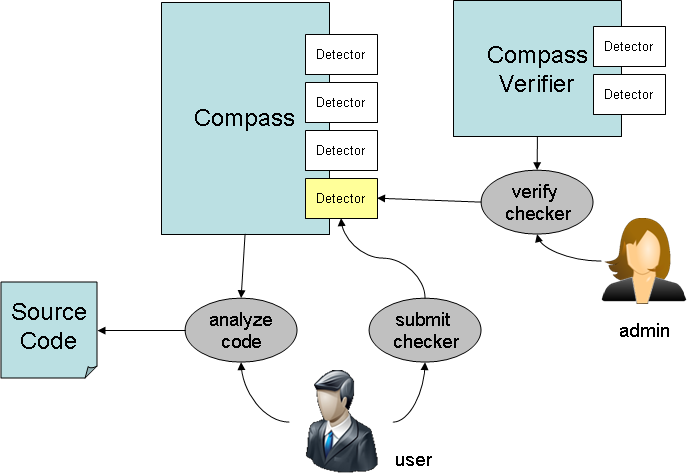
\includegraphics[width=4.5in]{compass_pic.png}
\caption{Compass Use Case}
\label{Compass_usecase}
\end{figure}

Either the same user or a different user/developer can also
implement and submit checkers to be built into Compass.
% Furthermore, a user may contribute with his own checkers that can be added to Compass. 
Since external users may contribute checker automatically via scripts, a verification of the 
validity and safety of these checkers is necessary. We provide a \emph{Compass Verifier}
that helps to check that all checkers are safe. Currently, the verifier is run by
an administrative person but may run automatically in the future.

%\section{Assumption of trust} 
\section{Trust Model}
By design we make a few assumptions about the use of Compass in order to define
a secure tool. We assume:
\begin{enumerate}
   \item For now, there is an assumption of trust in the person writing the checker. \\
      We use the \emph{Compass Verifier} as a way to double check the 
      checkers so that we can eventually weaken the level of trust assumed for people 
      writing checkers. However, the design of the \emph{Compass Verifier} is not likely to
      ever be robust enough to guarantee an automated proof of security for each checker.  
      Thus, we also assume that someone trusted will also review the checker.
      {\em not implemented: We expect that a digital signature (using a key mechanism) 
           is possible to associate a trusted reviewer with a review of 
           the checker together with a strong hash function that
           digitally signs the checker source code.}

   \item Since running \emph{Compass Verifier} is an optional part of building 
      the Compass executable, the person running these test is trusted. There are
      two ways to run the \emph{Compass Verifier} (see section \ref{sec:compass_verify}
    for details):
      \begin{itemize}
         \item Slow: once on each checker ({\tt make verify}). This mechanism
            tests all the files one checker at a time and thus can not miss 
            a file.  Note that even the counter examples are tests which can 
            be a problem when the counter example for the checker is detected
            as a violation for \emph{Compass Verifier}.  Counter examples for
            checkers have to be carefully written to not represent examples that
            violate \emph{Compass Verifier}.
         \item Fast: once on the union of all the checkers ({\tt make oneBigVerify}).
            This step forms a single file of all the checkers (and in-doing so can
            miss some files, and so is less secure).  It is mostly for testing 
            purposes.
      \end{itemize}

   \item The person building the Compass executable is trusted.

   \item The environment where the testing using Compass is done is trusted.

   \item Compass is designed so that the user running Compass need not be trusted.

\end{enumerate}

It is unclear at present how weak the assumption of trust on the compass checker developer 
can be and it may ultimately depend directly on the capabilities of the \emph{Compass Verifier}.


\section{Architecture}

\begin{figure}[thb]
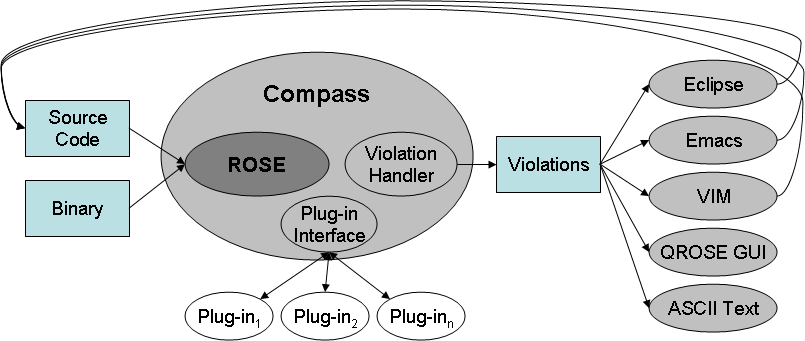
\includegraphics[width=6.0in]{compass_arc.png}
\caption{Compass Architecture}
\label{CompassArchitecture}
\end{figure}


Compass is a tool that allows users to implement checkers to locate and
report software defects.
Documentation of various kinds of software defects can be found in sources
such as the CERT Secure Coding Rules, Common Weakness Enumeration from MITRE, 
and other sources. Our focus is not to define new software defects but
rather to provide a platform that allows the easy implementation of defect
checkers.  Compass has been designed to be easy to extend, allowing users to 
implement their own custom checkers (custom source code analyses for
identifying defects), as shown in Figure~\ref{CompassArchitecture}. Compass supports
the implementation of both simple as well as more advanced defect
checkers. For the latter, Compass utilizes the ROSE infrastructure to
perform a wide range of general purpose program analyses, such as control
flow analysis, data flow analysis, program slicing, etc.


Compass is designed in a way that allows users who do not necessarily have
compiler backgrounds to utilize the ROSE infrastructure to build their
own analysis tools.
Compass is foremost an extensible open source infrastructure for the
development of large
collections of rules. Our current implementation supports automatic
defect checking, programming language restriction, and malware detection in
C, C++, and object code.
Support for Fortran is a new addition to ROSE and will be supported in
Compass in the near future.




\section{Design}

\begin{figure}[thb]
\hspace{-1.5in}
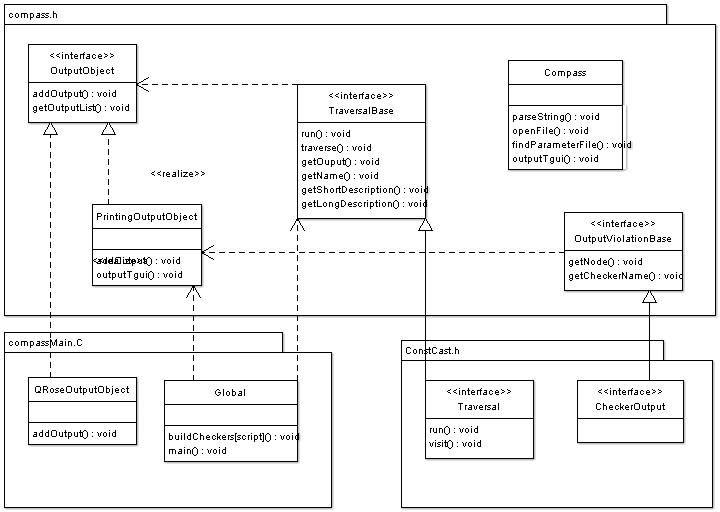
\includegraphics[width=7in]{compassdesign.png}
%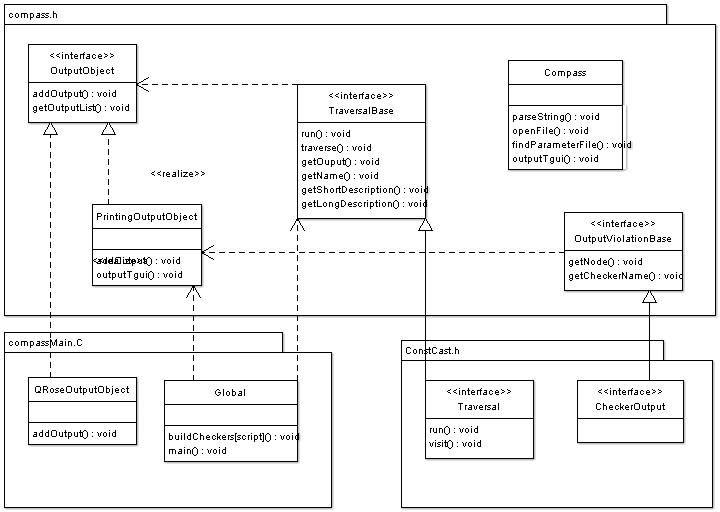
\includegraphics[width=6.0in]{compassdesign.png}
\caption{Compass Design}
\label{CompassDesign}
\end{figure}

Compass is designed to be easy to extend. Any user may write a checker and add it to
Compass. Figure~\ref{CompassDesign} illustrates the UML design decisions behind Compass.


Most of the functionality of Compass is in abstract classes hidden in the Compass
namespace within compass.h - a file within the compassSupport directory. The figure uses a
specific example, {\em ConstCast}, for illustration; Compass is designed to support a large
number of checkers (hundreds). All checkers, such as the {\em ConstCast} checker (illustrated in
figure~\ref{CompassDesign}), utilize the abstract classes to traverse a program with all
its nodes and to output violations found in that code according to the local algorithm.

CompassMain is the main executable that initially calls ROSE to parse a program. Then
\emph{buildCheckers} is called to load all checkers that are specified within a
configuration file. The configuration file allows users to turn on and turn off specific
checkers for their run-time analyses. However, the configuration file only permits
checkers to be loaded that were part of Compass at compile-time.

The main interface file compass.h contains the abstract classes \emph{TraversalBase} and 
\emph{OutputObject}. TraversalBase is the interface to ROSE, allowing a checker to
traverse the ROSE AST (program) and hence perform analysis on that AST. OutputObject aids
to output defects found by a specific checker. More functionality to handle e.g. file
input and parameters provided to Compass, is provided within the Compass namespace.

\section{Compass Verifier}

Compass must be safe, so that analyses and their results can be trusted. 
The {\em Compass Verifier} is used at build time to run a specific set of separate 
compass rules offer the source code of all the checkers.  For simplicity it runs in two
modes: fast, for checking specific named checker source files; and slow, for testing 
{\em all} checker source files.

\subsection{Threats} 

In order to define a complete design for security we outline the threats that
understand to be relevant. The main threats to the validity of Compass checkers are:
\begin{itemize}
\item \emph{Malicious User} \\ 
  A malicious user is an external user of Compass contributing a checker that performs malicious behavior.
\item \emph{Malicious Checker} \\ 
  Compass is extensible and new checkers can be added externally (users outside the main development group).
  A checker can be programmed arbitrarily using the C/C++ and assembly programming languages. 
  It is therefore possible for a skilled programmer to hide malicious operations within a
  checker.  Compass must prevent checkers with malicious behavior to be part of the
  Compass system. Threats are:
   \begin{itemize}
      \item {\bf exfiltration} \\
         A checker should act in a secure way with the input files it is given.
         Securing the inputs to Compass (e.g. the inputs to each checker) from 
         exfiltation is a first priority. Allowing a checker to scan the host 
         machine to exfiltrate arbitrary data (this is a threat that any secure
         software will have).
      \item {\bf modification of filesystem} \\
         A checker should be side-effect free, or have only well defined side-effects, 
         but a malicious checker could modify or erase parts of the accessible file 
         system (e.g. deleting whole directory structures).
%     \item {\bf others ??? ...}
   \end{itemize}

\item \emph{Malicious Compass} \\
    Since Compass is built from ROSE, it is possible to modify compass (or any checker) 
    to generate source code that could be compiled to replace the existing executable
    (there are some constraints here) or regenerate the source code to replace the 
    existing source code or perhaps just provide an alternative copy of the source code.
    This indirect transformation of the input code is a threat.

\item \emph{Source Code Replacement} \\ It should not be possible for users to exchange the
    source code of checkers within a running system, i.e. Compass cannot implement dynamic
    loading of checkers. Such a feature would compromise its safety.

\item \emph{Binary Replacement} \\ Another threat is the replacement of a valid Compass
    checker with a modified malicious version within a binary release of Compass.
    Therefore, Compass should be aware if parts of itself were modified and should not
    execute.

\end{itemize} 

%\subsection{Safety Handling}
\subsection{Mitigation of Threats}

Compass is designed to be safe. The Compass Verifier is a stable separate copy of Compass
that contains only a few checkers to check (external and internal) user delivered checkers
for safety.  We have hopefully designed Compass in a way that it addresses the threats
mentioned above:
\begin{itemize}
\item \emph{Malicious User} \\ Initially, we permit only trusted individuals to add new
    checkers to Compass. Once the verification process is matured, we will extend this
    policy to allow less trusted users to contribute to Compass. A goal will be to allow
    arbitrary users to contribute checkers, however, a review of the whole Compass design
    (and the {\em Compass Verifier} especially) will be required to define required trust
    levels for user/developers who implement checkers.
\fixme{We might define trusted and untrusted checkers as a way to have checkers from
       arbitrary users, but mark them as untrusted.}

\item \emph{Malicious Checker} \\ To prevent Compass from executing malicious code, the Compass
    Verifier executes its own checkers on any user defined checker that is being
    considered to be added to Compass. Currently, the Compass Verifier contains three checkers:
   \begin{itemize}
      \item \emph{fileReadOnlyAccess} ensures that a user defined checker performs no write
         or execute operations on files.
      \item \emph{allowedFunctions} is a {\em white list} of function calls permitted in
         a checker. This list contains functions that are trusted and hence considered
         safe when integrated to Compass.
\fixme{This is not yet implemented as a white list and is instead currently a black list; called: forbiddenFunctions.}
      \item \emph{noAsmStmtsOps} searches for assembly instructions in a checker and flags
         and reports all cases as unsafe.
      \item To avoid modifications of the AST for the purpose of allowing other checkers
         to pass, the AST should not be modified (this should extend to all the
         program analysis graphs generated and used by other checkers).
         {\em This is not implemented yet.} 
\end{itemize}

\item \emph{Malicious Compass} \\
    Since Compass does not generate code, it can not be used to modify the input software
    (source code or binary) or generate a new copy that could be confused with the input.
    However, future versions of Compass make make transformation to introduce greater
    levels of security; fix flaws, mitigate specific forms of threats, etc.  It will be
    important to make sure that such transformation can not change the behavior of an
    input code to make the modified input code malicious.  Current proposed approaches
    would build a patch which would have to be inspected by a trusted developer before
    it would be applied to modify the input code.

\item \emph{Source Code Replacement} \\ Checkers can only be added at compile time to
    Compass, not at run-time. This means that checkers (meaning the source code) cannot be
    exchanged against unsafe versions at run-time. Furthermore, we allow only the Compass
    tool builder (admin) to build versions of Compass that must pass the Compass Verifier.

\item \emph{Binary Replacement} \\ 
    Our goal is to perform a strong hash (e.g. Secure Hash Algorithm - SHA2) as a 
    checksum on all the checkers
    part of the binary Compass distribution before Compass is executed. In this way
    Compass will not run if parts of it were modified. {\em This is not implemented yet.}
\fixme{We should describe the policy for allowing SHA2 to be verified. Where the SHA2
    results for checkers would be published (e.g. web site), etc.}

\end{itemize} 


%The above list contains an important subset of checkers that enforce Compass checkers to be safe. 
%Additional checkers can easily be added to that list.
%In the future, a checker submitted to Compass, should go first through the automatic verifier, before it is either 
%added to Compass or denied.  


\section{Future Work}

    Currently we are engaged in design reviews with CERT, we expect that this will lead to 
improvements in the security to support a key based approach to a trusted execution of
tools built within the compass infrastructure, including Compass itself.



\newpage

\chapter{Using Compass}

\section{Running Compass}

    Compass is currently distributed as part of ROSE, and represents one
of many tools that can be built using the ROSE open compiler infrastructure.
Compass resides in the {\tt ROSE/projects/compass}.  As part of building ROSE
Compass will be automatically built in the Compass directory.  Running compass
is a matter if typing {\tt compassMain} and handing in a number of options.
The {\tt compassMain} program acts just like a compiler so it is appropriate
to hand it the same options required to compile your source file (e.g {\tt -I}
directory paths and a source file.  Compass will figure out the language from
the source file suffix.  Using the {\tt --help} option will provide a more
complete list of options available to ROSE based tools.  See also the section
of this chapter on the include/exclude options for path and file names as
these will permit the output from header files to be tailored.


\section{Output from Compass}

   Output from compass can be generated in a number of forms, the default is
ASCII text output of the messages about rule violations with the source code
position in {\it GNU standard source code position format}.  This form can be
used to interact with external tools (e.g. Emacs) to permit alternative
interface to Compass.  Mechanisms available include:

\begin{itemize}
   \item Emacs: \\
         Detecting errors while you type \ref{compassEmacs} and \ref{Compass_Emacs_Screenshot}.
   \item Vim 7: \\
         Compass can work with Vim 7's QuickFix commands to
         highlight source lines with error messages \ref{Compass_VIM7_Screenshot}. 

   \item CompassGUI: \\
         There is also a Compass GUI for reviewing Compass output and interactively
         rerunning compass and sifting through the output while relating them to the source
         code \ref{Compass_GUI}. This work uses the QRose library produced at Imperial College
         London by Gabriel Coutinho, as part of their development of FPGA tools using ROSE.
         QRose is based on the Qt library and provides a wide number of ROSE aware components
         to make the development of GUIs for ROSE based tools easy.  The source code for the 
         Compass GUI is provided, but this work is unfinished (and required the QRose library
         available from Imperial).

   \item ToolGear post-processing: \\
         Output in XML permits the use of ToolGear (LLNL tool available on the web) for
         viewing Compass generated output.  This mechanism is particularly useful for reviewing
         the results of nightly builds (and associated runs of large projects using
         Compass). See figure \ref{Compass_ToolGear_Screenshot}

   \item ASCII output: \\
         Output in ASCII format is of the form shown in \ref{Compass_ASCII_Output}.  This
         form permits the connection to multiple external tools (the Emacs interface reads
         the ASCII output format directly).
 
\end{itemize}


\begin{figure}
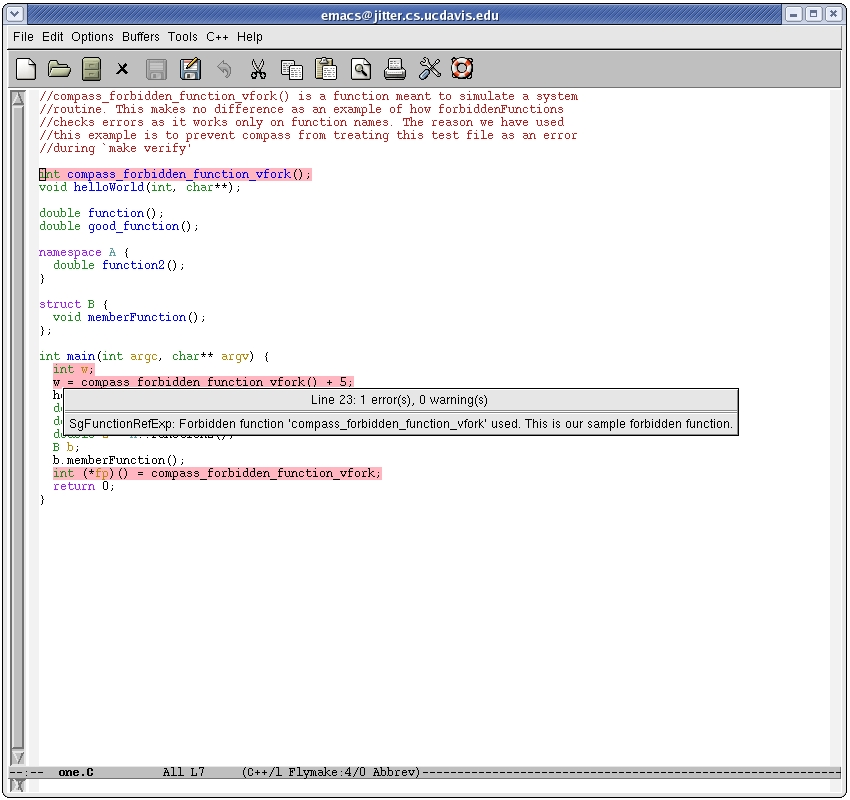
\includegraphics[width=7in]{emacs_screenshot.jpg}
\caption{Compass error messages integrated into Emacs}
\label{Compass_Emacs_Screenshot}
\end{figure}

\begin{figure}
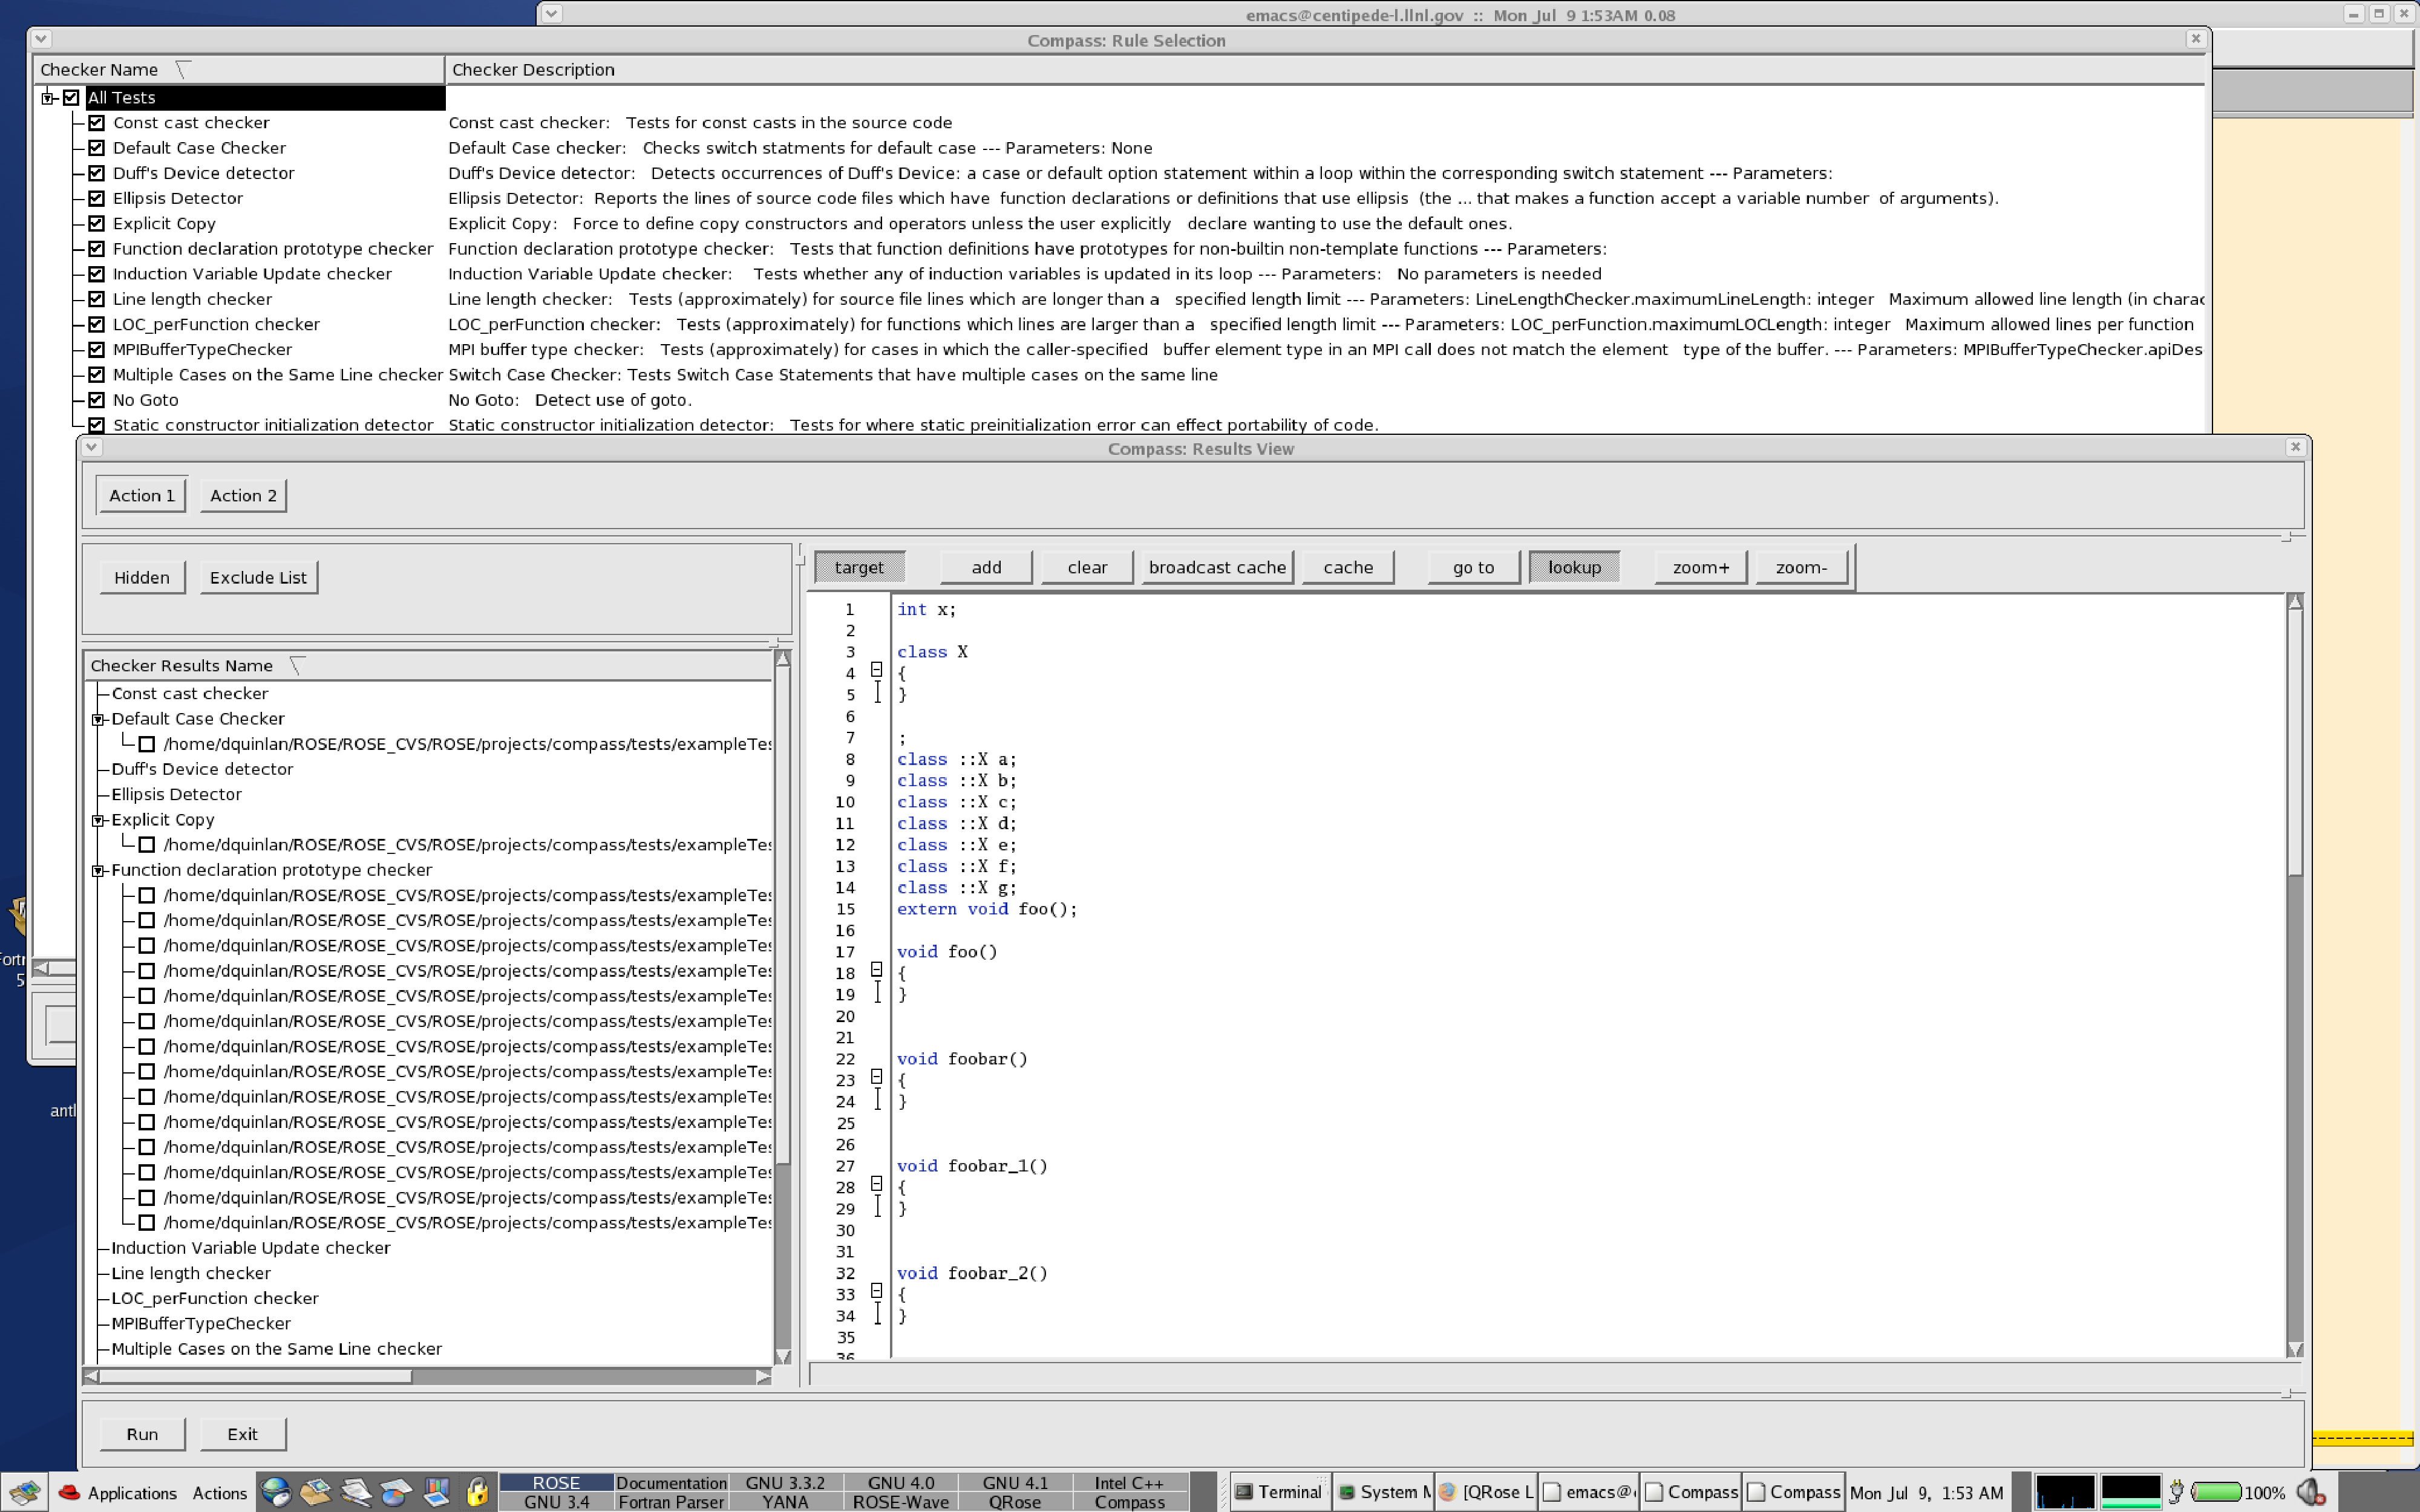
\includegraphics[width=7in]{CompassScreenshot.pdf}
\caption{Compass GUI for interpretation of rule violations}
\label{Compass_GUI}
\end{figure}

\begin{figure}
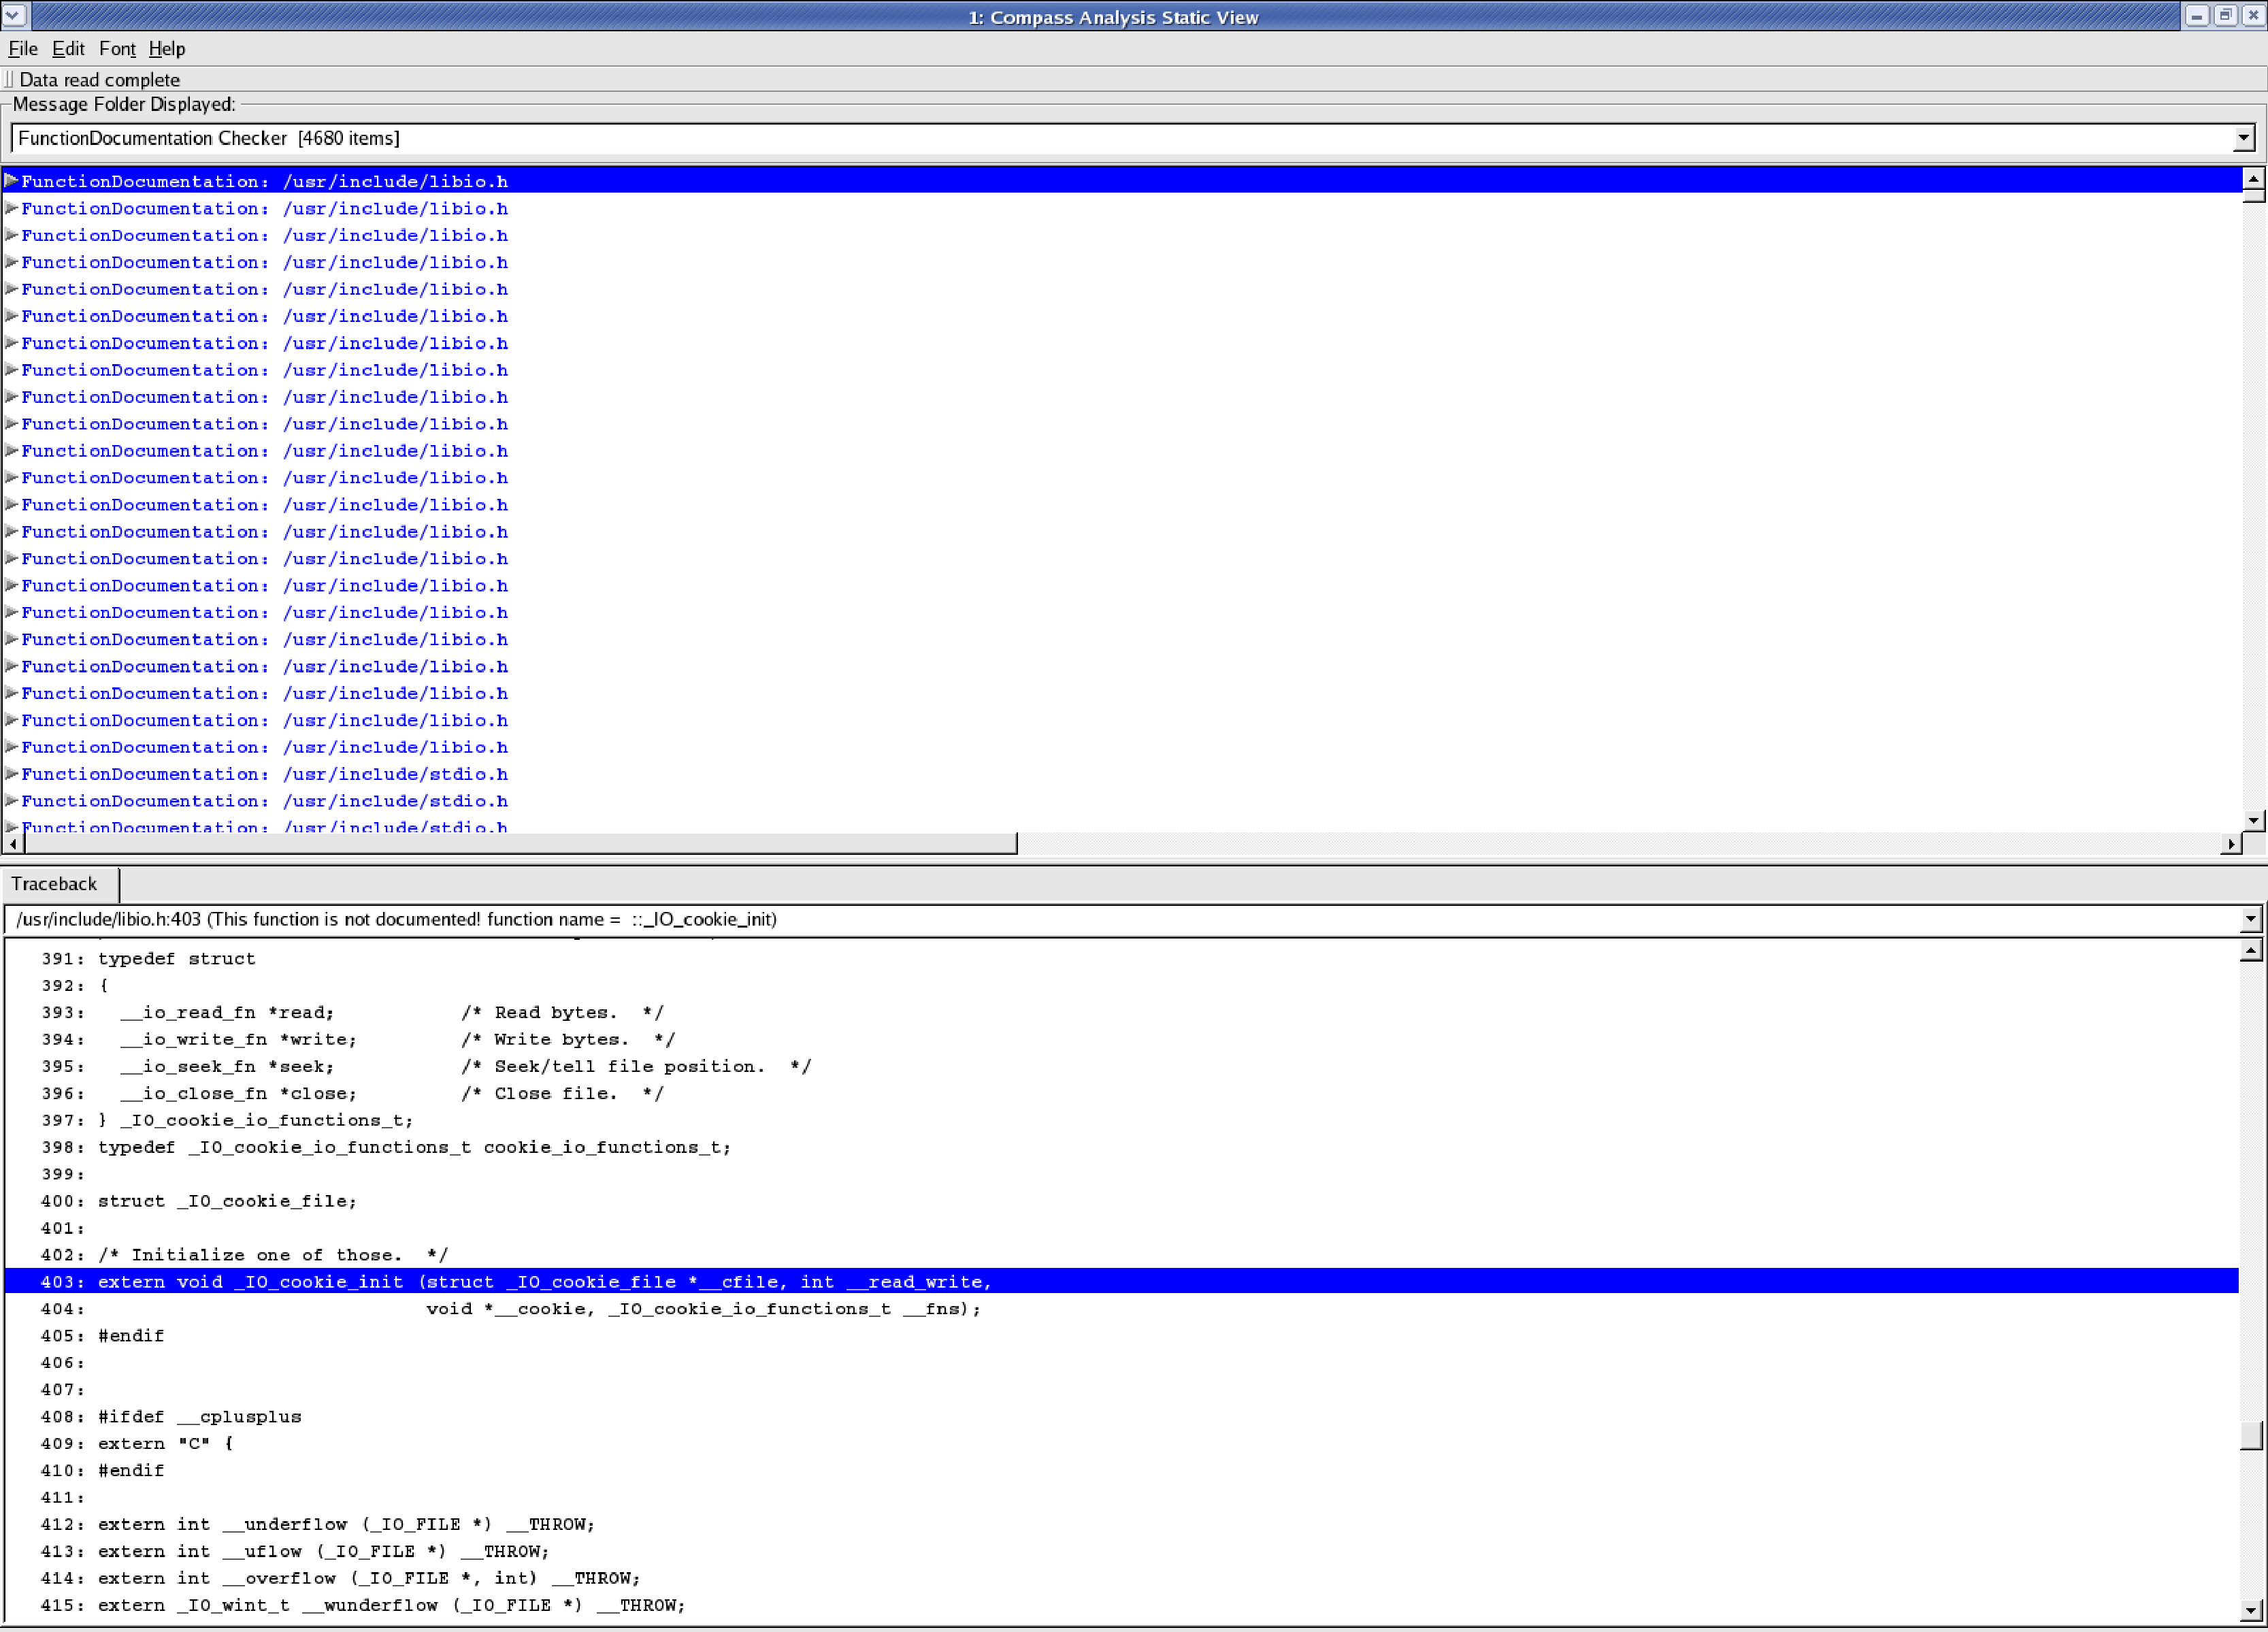
\includegraphics[width=7in]{ToolGear_gui_compass_01.pdf}
\caption{Processing of XML Compass output using ToolGear}
\label{Compass_ToolGear_Screenshot}
\end{figure}

\begin{figure}
{\scriptsize
\begin{verbatim}
LocalizedVariables: /home/ROSE/projects/compass/tests/Cxx_tests/test2006_117.C:30.5: Variable pmNull does not seem to be used.
FunctionDefinitionPrototype: /home/ROSE/projects/compass/tests/Cxx_tests/test2006_123.C:27.1-10: matching function prototype not available
LocPerFunction: /home/ROSE/projects/compass/tests/Cxx_tests/test2006_117.C:23.1-20: This function has too many lines of code :: LOC = 14 > 10
MagicNumber: /home/ROSE/projects/compass/tests/Cxx_tests/test2006_117.C:33.14: Occurrence of integer or floating constant.
MagicNumber: /home/ROSE/projects/compass/tests/Cxx_tests/test2006_117.C:36.14: Occurrence of integer or floating constant.
MagicNumber: /home/ROSE/projects/compass/tests/Cxx_tests/test2006_117.C:37.14: Occurrence of integer or floating constant.
FunctionDocumentation: /home/ROSE/projects/compass/tests/Cxx_tests/test2006_123.C:27.1-10: function is not documented: name =  ::main
FunctionDocumentation: /home/ROSE/projects/compass/tests/Cxx_tests/test2006_123.C:9.10: function is not documented: name =  ::X < int , int , 10 > ::f
FunctionDocumentation: /home/ROSE/projects/compass/tests/Cxx_tests/test2006_123.C:12.10: function is not documented: name =  ::X < int , int * , 5 > ::f
FunctionDocumentation: /home/ROSE/projects/compass/tests/Cxx_tests/test2006_123.C:16.10: function is not documented: name =  ::X < int * , float , 10 > ::f
\end{verbatim}
}
\caption{Example of ASCII output from Compass. }
\label{Compass_ASCII_Output}
\end{figure}



\subsection{Using Compass With Emacs}

\label{compass::emacs}

Compass as a checker is most useful when the user is notified as early as possible
when he violates a desired software property. Although for many purposes it is
sufficient to run Compass separately; it is possible to use compass
seamlessly when developing in emacs. By using an emacs extension called {\em flymake} together
with Compass erroneous lines can be highlighted while programming, and the relevant error messages displayed 
in a dialog. Syntax errors from ROSE will be displayed as well, see figure \ref{Compass_Emacs_Screenshot}.

Much thanks for David Svoboda at CERT at CMU for first configuring Flymake to work with
Compass and demonstrating the idea.  It has provided a great way to check code using
compass and its use in Emacs has stimulate a number of ideas that have made their way
back into Compass.

\subsubsection{Emacs .emacs Code Requirement}

   Figure \ref{compassEmacs} shows the code that is required to be added to the {\tt .emacs}
file.  A copy of this code is available in the compass source directory in the file
{\tt emacs\_compass\_config.el}.

\begin{figure}
{\scriptsize
\begin{verbatim}
; New Compass support for Emacs using version 22 of Emacs and Flymake.
; Comment out these two lines to use older version of emacs.
(require 'flymake)
(setq flymake-allowed-file-name-masks (cons '(".+\\.C\\'" flymake-simple-make-init flymake-simple-cleanup flymake-get-real-file-name) flymake-allowed-file-name-masks))


(defun flymake-master-make-header-init ()
  (flymake-master-make-init 'flymake-get-include-dirs
			    '("\\.C\\'" "\\.c\\'")
			    "[ \t]*#[ \t]*include[ \t]*\"\\([[:word:]0-9/\\_.]*%s\\)\""))

(add-hook 'find-file-hook 'flymake-find-file-hook)

(setq flymake-log-level 3)
(setq flymake-no-changes-timeout 0.5)

(defcustom rose-source-tree "/home/dquinlan/ROSE/NEW_ROSE/" "Location of top of ROSE source tree")
(defcustom rose-build-tree "/home/dquinlan/ROSE/ROSE_CompileTree/LINUX-64bit-3.4.6/" "Location of top of ROSE build tree")
(defun add-buildfile-dir-for-rose ()
  (let ((source-dir-name (file-name-directory buffer-file-name)))
    ;(message "%S" `(source dir ,source-dir-name))
    (if
      ; (string-equal rose-source-tree (substring source-dir-name 0 (length rose-source-tree)))
        (string-equal rose-source-tree (substring source-dir-name 0 (min (length source-dir-name) (length rose-source-tree))))
        (let ((buildfile-dir (concat "../../../../../../../../../../../../../../../../../../../" rose-build-tree "/" (substring source-dir-name (length rose-source-tree)))))
        ; (message "%S" `(buildfile-dir ,buildfile-dir))
        ; (set-variable 'flymake-buildfile-dirs (cons buildfile-dir flymake-buildfile-dirs) 'local))
          (set-variable 'flymake-buildfile-dirs (append (mapcar (lambda (dir) (concat buildfile-dir "/" dir)) flymake-buildfile-dirs) flymake-buildfile-dirs) 'local))
      (progn
        ;(message "%S" `(bad-prefix))
        source-dir-name))))
(defun set-rose-source-dir (dir) "Set the top of the ROSE source tree to use with Flymake" (interactive "DThe top of the ROSE source tree: \n")
  (setq rose-source-tree dir 'local)
  (add-buildfile-dir-for-rose))
(defun set-rose-build-dir (dir) "Set the top of the ROSE build tree to use with Flymake" (interactive "DThe top of the ROSE build tree: \n")
  (setq rose-build-tree dir 'local)
  (add-buildfile-dir-for-rose))

(add-hook 'find-file-hook 'add-buildfile-dir-for-rose)

;(list "make"
;;  (list "-s" "-C" "/home/dquinlan/ROSE/NEW_ROSE/developersScratchSpace/Dan/EmacsCompass_tests/"
;    (list "-s"
;   (list "-s -C" "`pwd | sed 's@^/home/dquinlan/ROSE/NEW_ROSE/@/home/dquinlan/ROSE/ROSE_CompileTree/LINUX-64bit-3.4.6/@'`"
;	   (concat "CHK_SOURCES=" source)
;	     "SYNTAX_CHECK_MODE=1"
;		   "check-syntax"))

(global-set-key [f3] 'flymake-display-err-menu-for-current-line)
(global-set-key [f4] 'flymake-goto-next-error)

\end{verbatim}
}
\caption{Addition to .emacs when integrating Compass into emacs. }
\label{compassEmacs}
\end{figure}

\subsubsection{Emacs Version Requirement}

Emacs version 22 or newer is required to take advantage of the emacs integration of
Compass. Before using Compass a 3 step process must be followed:
\begin{itemize}
   \item Add the text in figure \ref{compassEmacs} (in {\tt ROSE/projects/compass/emacs\_compass\_config.el}) to .emacs
   \item Change /path/to/makefile in figure \ref{compassEmacs} to the path to the project you are editing in Compass
   \item Add a 'check-syntax' rule to the makefile of the project that you are working
   on in Compass. This rule should compile all the files you want Compass to check 
   or all files that you are editing with Compass as the compiler.
\end{itemize}

Figure \ref{compassEmacs} shows the needed changes in .emacs for integrating
Compass. The last two lines are the most interesting lines since they introduce two
shortkeys. [f3] can be clicked in order to display all errors for the current line while
[f4] will move the cursor to the next error. 

A short explanation of the code in figure \ref{compassEmacs} is that the first line will require 
the flymake extension to be available upon
loading emacs while the second line will load the find-file-hook and flymake-find-file-hook
functions. The "setq" sections that follows runs Compass for all files that are being edited
that has the c and C extensions. The ``list'' section tells flymake to execute the check-syntax
rule in the makefile. 

\subsubsection{Example check-syntax rule}


\begin{figure}
\begin{verbatim}
one: inc.h one.C
        g++ -c one.C
\end{verbatim}
\caption{Example makefile before the Compass addition  }
\label{beforeProjectCheckRule}
\end{figure}


\begin{figure}
\begin{verbatim}
one: inc.h one.C
        g++ -c one.C
		
check-syntax: inc.h one.C
        /path/to/compass/executable/compassMain -c one.C
\end{verbatim}
\caption{Example makefile after addition to support integration of compass  }
\label{projectCheckRule}
\end{figure}


Figure \ref{beforeProjectCheckRule} shows an example makefile that compiles a file
"one.C" using g++. If "one.C" is edited using emacs the addition of the "check-syntax"
rule is needed, as shown in figure \ref{projectCheckRule}.

\subsection {Using Compass With Vim}
%--------------------------------------------
Compass can be used with Vim 7's QuickFix commands to display warning
messages and highlight the source lines in question. A compass compiler
plugin (compass.vim as shown in Figure \ref{compassVim7})  has
been provided for Vim to parse the warning messages outputted by Compass.

Steps to make Compass work with Vim 7
\begin{itemize}
\item Save compass.vim into ~.vim/compiler.  Create the target directory if it
does not exist.
\item Download errormarker.vim from
http://www.vim.org/scripts/script.php?script\_id=1861 and save it
into .vim/plugin . Again, create the target directory first when it does not
exist.
\item Change your Makefile to use an installed compassMain as the compiler
to compile your code.
\item Use quickfix features of Vim 7 as documented at
http://vimdoc.sourceforge.net/htmldoc/quickfix.html. Some frequently used
commands are:
  \begin{itemize}
   \item Specifying the compass plugin to use by typing a command :compiler compass
   \item Open your source code using gvim and set the compiler to Compass by
   \item Compile you code using compassMain, type :make
   \item Display current message, type :cc
   \item Display all messages, type :clist
   \item Jump to next message, type :cnext
  \end{itemize}
\end{itemize}
%-------------------------------
\begin{figure}[!htp]
{\scriptsize
\begin{verbatim}
" Vim compiler file
" Compiler:     ROSE Compass 0.9.2a
" Maintainer:   Chunhua Liao <liao6@llnl.gov>
" Last Change:  2008 Apr. 3
"
if exists("current_compiler")
  finish
endif
let current_compiler = "compass"

if exists(":CompilerSet") != 2          " older Vim always used :setlocal
  command -nargs=* CompilerSet setlocal <args>
endif

" single line warning
" multiple line warning, %W, %C continue line %Z end of multiple line
CompilerSet errorformat=%s:\ %f:%l%.%c:\ %m,
         \%s:\ %f:%l%.%c-%*\\d:\ %m,
         \%s:\ %f:%l%.%c-%*\\d%.%*\\d:\ %m,
         \\\"%f\"\\,\ line\ %l%*\\D%c%*[^\ ]\ %m
"some notes about the error/warning message format
"Official guide: http://vimdoc.sourceforge.net/htmldoc/quickfix.html#error-file-format
" Each new rule start with a leading \ unless it is the first rule in the
" first line
"  %f: filename %l: line number %c: column number, only one is permitted %m
" actual error/warning message \ :matching a space
"  %*\\d: matching any number

\end{verbatim}
}
\caption{A compiler plugin for Vim 7 compass.vim}
\label{compassVim7}
\end{figure}
%-------------------------------
Figure ~\ref{Compass_VIM7_Screenshot} shows an example of Compass error
messages integrated into Vim 7.
\begin{figure}[!htp]
\centering
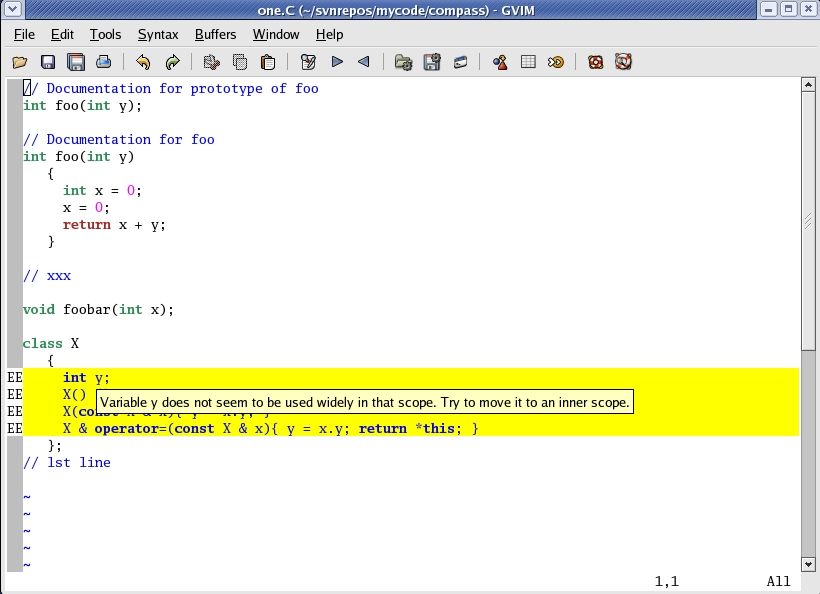
\includegraphics[width=0.7\textwidth]{compass_vim7.jpg}
\caption{Compass error messages integrated into Vim 7}
\label{Compass_VIM7_Screenshot}
\end{figure}

%-------------------------------
\clearpage
\section{How To Write A New Checker}

\subsection{Creating A Skeleton}

Compass has scripts for creating a skeleton for a new Compass
checker. This skeleton can be easily adapted to write all checkers.

Follow these steps to generate a checker skeleton:
\begin{enumerate}
   \item Enter a directory where you want the directory of your checker to be created
   \item Execute {\tt ROSE\_SRC\_DIR/projects/compass/compass\_scripts/gen\_checker.sh $<$name of your checker$>$}
\end{enumerate}

The results of executing gen\_checker.sh script is that a new directory name 
``multipleCasesOnSameLine''
(name of your checker in camel case) is created with the following files:

\begin{verbatim}
compass.C           multipleCasesOnSameLine.C
compass.h           multipleCasesOnSameLineDocs.tex
compass_parameters  multipleCasesOnSameLine.h
compassTestMain.C   multipleCasesOnSameLine.inc
Makefile            multipleCasesOnSameLineMain.C
Makefile.am         multipleCasesOnSameLineTest1.C
\end{verbatim}

Some of these files (compass.[Ch], compass\_parameters, and compassTestMain.C)
are copied from the compass\_template\_generator directory; while others are
generated (multiple*, Makefile, Makefile.am)

It is suggested that you keep the following in mind when using gen\_checker.sh:
\begin{itemize}
\item
   It is advised that you do not invoke the script gen\_checker with words
   like checker, detector, tester, etc. Adding these verbs at the command
   line means that these words are added as suffixes into the
   directory-name. Which will make it redundant, as the compass project is
   about writing style-checkers!
\item
   Some of the files have read-only permissions and are intended only for
   such use. Please do not change the permissions of these files.
\item
Advanced: The file `multipleCasesOnSameLine.inc' is used to pass in custom LDADD lines
to the Make environment on a per checker basis. The LDADD line specified in
this file will be added verbatim to the compass makefile.

\end{itemize}

\subsection{Integrating New Checkers Into Compass}
\label{howToIntegrateNewCheckers}

The process for integrating a new checker into Compass has been automated. These directions
are meant for checkers generated using gen\_checker.sh.

The steps to integrate a new checker is
\begin{enumerate}
   \item Create a tar file of the directory tar -zcvf  $<$name of your checker$>$.tar.gz $<$name of your checker$>$
   \item Add $<$name of your checker$>$ to CHECKER\_LIST
   \item Copy $<$name of your checker$>$.tar.gz to ROSE\_SRC\_DIR/projects/compass/compassRepository/
   \item Enter ROSE\_BUILD\_DIR/projects/compass/ 
   \item Execute 'make regenerate'
   \item After running 'make regenerate' in the build tree then you may run make as usual.
   \item %Before executing compassMain or any Make rule that uses compassMain, 
	Examine the RULE\_SELECTION file in projects/compass such that it 
	reflects your most recent additional checker(s) choice of execution at
	run-time; the default setting is ``on''. Please refer to section 
	~\ref{ruleselection}.
\end{enumerate}

In the Makefile, the compass\_submission\_setup.sh handles adding/updating a Compass checker into
an existing Compass source tree. ``regenerate'' is an argument that instructs the script to perform a 
read-only operation on the file CHECKER\_LIST in your projects/compass directory. This file contains 
a list of checkers that will be integrated by compass\_submission\_setup.sh.

The file `CHECKER\_LIST' can use the `\#' comment delimiter at the beginning of
any checker name to remove that checker from compilation. The hash mark may
only appear at the beginning of the line. The compass\_submission\_setup.sh
script must be run again with the ``regenerate'' option if any checkers are
commented out. {\bf Note that no space is permitted between the `\#' and the name
of the checker.}

As stated previously, the compass\_submission\_setup.sh script handles
adding/updating Compass checkers into the compass source tree (usually located
at ROSE/projects/compass). It does this by generating the necessary files
to compile Compass with the checkers located in $<$COMPASS SUBMIT DIR$>$. These
files are:

\begin{itemize}
\item {\bf CHECKER\_LIST}: 
	a file that keeps a running list of all checkers seen by 
	compass\_submission\_setup.sh.
\item {\bf \${CHECKER}/\${CHECKER}.makefile}: An individual Make file is
	generated per checker in its directory such that it may be separated
	for individual development before being reincorporated with Compass.
\end{itemize}
%
The \${CHECKER}.makefile file is generated such that any checker may be copied
out of the source tree projects/compass and worked on separately. This feature
speeds up development of single checkers as is removes the requirement to
rebuild the entire compassMain tool.

Many automatically generated files required for the build of Compass are 
generated in the build tree. Rules for the generation of these files are found
in the automake Makefile.am file in the Compass source tree directory 
projects/compass. These file include:

\begin{itemize}
\item {\bf CHECKER\_LIST\_WITHOUT\_COMMENTS}: a version of CHECKER\_LIST
	that expands in two columns those checkers built as part of Compass
	in camel case starting with a lower-case letter and an upper-case
	letter respectively.
\item {\bf compass\_makefile.inc}: a Make include file that sets the Make environment
	with the information for each checker. This environment specifies
	the rules needed to compile each checker object, make the
	documentation, and test all checkers together or separately.
   {\bf compass\_makefile.inc}: provides the following Make rules: 
	(note \$\{CHECKER\} is the name of a checker directory i.e. 
	doNotDeleteThis)
   \begin{itemize}
      \item {\bf docs}:  makes the documentation

      \item test\$\{CHECKER\}: tests a single checker, a single rule is provided
		      per checker.

      \item testAllCheckersSeparately: tests all checkers separately as a batch.

      \item archive\$\{CHECKER\}: -- tar \& gzips a single checker directory in 
		projects/compass/\$\{CHECKER\} to 
		projects/compass/compassRepository/\$\{CHECKER\}.tar.gz

      \item archiveCheckers: archives all checkers (uncommented in CHECKER\_LIST)
                projects/compass to
                projects/compass/compassRepository/\$\{CHECKER\}.tar.gz
   \end{itemize}

\item {\bf checkers.h}: An automatically generated file needed by compassMain.C that 
	contains a list of \#include directives for each checker header .h file.

\item {\bf buildCheckers.C}: An automatically generated source file needed by 
	compassMain.C to build the Compass checker traversals.

\item {\bf compassCheckerDocs.tex}: A Latex include file that inputs each checker .tex
	documentation file into the compass.tex document.

\item {\bf compass\_parameters}: The concatentation of individual checker parameter files
	to be used with compassMain.

\end{itemize}



\section{Including/Excluding Checkers in the Compass Build Process}
\label{CompassBuildProcess}

   This section describes how to select which of the checkers to integrate into Compass
out of all the checkers available in source form in the Compass source directory. For
security reasons Compass uses this static build process since it is a central goal
of Compass that it should run as a trusted part of a project's build process. If the
integration of checkers had been automatic through a dynamic plugin mechanism it
would be hard to ensure that the dynamic list of checkers was secure, but for a 
static list of trusted checkers this is possible.

In order to integrate a checker into Compass the user must:
\begin{itemize}
   \item Add the name of the checkers directory in the CHECKER\_LIST in the compass
      source directory
   \item Run {\tt make regenerate} in the Compass build directory
\end{itemize} 
If a user or developer intends to integrate a new checker into the Compass source
tree refer to section \ref{howToIntegrateNewCheckers}.

Usually the CHECKER\_LIST is only modified when a user or developer wants to 
add a new checker or select a subset of trusted checkers.  Checkers can be
commented out using a {\tt \#}, no space is allowed between the {\tt \#} 
and the checker name.


\section{Including/Excluding Checkers During Compass Execution}
\label{ruleselection}

   This section describes how to execute a subset of the checkers provided in the build
process (see section \ref{CompassBuildProcess}). This process is significantly more
interactive than defining what checkers to include in the Compass build process.
Since it is not unheard of that rules implemented by different checkers can be  
mutually exclusive or even contradicting this mechanism is essential for selecting the
subset of checkers that are interesting for a specific program that is checked.
Separate projects of developers could easily have their own RULE\_SELECTION file
to permit high levels of customization in the use of a Compass tool containing
a large number of checkers (e.g. for different languages).

   When used with the Emacs interface this provides a simple way to turn on and off
specific checkers by editing a single file (RULE\_SELECTION).  The name of this
file is specified in the {\tt compass\_parameters} file, this name may be changed.
The directories searched are: current directory, user home directory, and Compass
source tree (respectively).

\begin{verbatim}
   Compass.RuleSelection=RULE_SELECTION
\end{verbatim}


In order to select a checker to run the user must:
\begin{itemize}
   \item Add a line '-:$<$name of checker$>$' in a file called RULE\_SELECTION. 
   \item If a line  '-:$<$name of checker$>$' already exist the '-' can be modified into
a '+' to enable the checker or into a '-' to disable a checker.
\end{itemize}
It is required that every checker integrated into the Compass build is mentioned in
the RULE\_SELECTION.


\section{Including/Excluding Paths and Filenames with Compass}

    Compass permits paths and filenames to be specified for inclusion/exclusion
in reporting checker rule violations.  Run {\tt compassMain --help} to see
the commandline options.  Numerous other commandline options provided for all
tools build using ROSE may also be relevant.



\section{Checking Security Properties of Checkers}
\label{sec:compass_verify}

    Compass is designed for extensibility while providing the security for
the codes being checked.  To support this Compass provides a simple
mechanism for verifying specific properties of the checkers used in Compass.
Compass implements a specific small number of checkers that are used for checking
the checkers in Compass.  The directory compassVerify contains the implementation
of this subset of Compass that is used on itself.  These checkers may not
be modified and in the future MD-5 checksums will be provided to ensure the
integrity of this subset of Compass.  To verify the compass checkers run:
\begin{itemize}
   \item {\tt make verify} \\
        This makefile rule runs the compassVerify/compassMain on all the source files in
    all the checkers directories in Compass.  Because it runs compass on so
    many separate
    files this step can take a long time.
   \item Or {\tt make oneBigVerify} \\
        The makefile rule runs the compassVerify/compassMain on a single generated file
    built from all the checker source files and is particularly quick to run.
\end{itemize}



\section{Testing Compass and its Checkers}

   The {\tt tests} directory contains directories of tests that
are language specific:
\begin{itemize}
   \item C\_tests \\ 
         This directory contains a Makefile which will use the ROSE C test codes 
         to test Compass.
   \item Cxx\_tests \\ 
         This directory contains a Makefile which will use the ROSE C++ test codes 
         to test Compass.
\end{itemize}
To run these tests type {\tt make check} at any level on the Compass directory
hierarchy of the build tree.





\newpage

\chapter{Using Compass GUI}

Compass has a GUI available for exploring the checker warnings for either the compilation
of a single source file or the compilation of a whole project. This GUI allow the user to
interactively select checkers, run those checkers on the source file(s) of 
interest and display the source location of each violation. As a user convenience the
interface will either display the violating source region in a text editor or a 
non-editable display window.

The Compass GUI is located in the 'projects/compass/tools/compass/gui' directory of the
ROSE distribution. The Compass GUI is build as part of the standard Compass build when
ROSE is configured with qt4. In order to enable simple compilation of whole projects using
one-button clicks in the Compass GUI ROSE must be configured with sqlite3 as well.

\section{Running Compass GUI on a Single File}
\label{runningCompassGUISingleFile}

Before running the Compass GUI on a single file  the files listed 
in \ref{usingCompassInstallation} must be available and the environment variable 
'\$COMPASS\_PARAMETERS' must specify which compass\_paramaters file to use. CompassGUI can
then be invoked as a normal compiler like e.g:
\begin{verbatim}
compassMainGui -o ex1 ex1.C
\end{verbatim}
If it is not desirable to export the '\$COMPASS\_PARAMETERS' variable a shorthand is:
\begin{verbatim}
env COMPASS_PARAMETERS=/location/of/compass_pramateres   compassMainGui -o ex1 ex1.C
\end{verbatim}

\section{Running Compass GUI on an Autotools Project}

A goal of this section is to show how to run the compass checkers on a whole project (like e.g ROSE) 
using a one button click in the Compass GUI and present an easy interface for exploring the violations
as found during the build. This interface is currently limited to sequentially building the
project and it requires ROSE to be configured with sqlite3. The Compass GUI does not try to replace the 
build system; it simply captures how the build system compiles the source files for a specific version of the 
project. Although there is no guarantee that this will work when the source code changes it is reasonable to 
expect the capturing of the build system should be the same as the code evolves as long as no changes are done 
to the build system.

These instructions can apply to Autotool projects as well as projects build in other build 
systems, but the shorthands used here for discerning the build system are specific for Autotools.


\subsection{Capturing a Build System State}

\fixme{Document: that this requires --with-sqlite3}

The first step of running the Compass GUI on an autotools project is to figure out how the build system
works. Capturing the build system state is done with the 'buildInterpreter' tool provided in the Compass
distribution in the 'projects/compass/tools/compass/buildInterpreter' directory. 

In order to facilitate capturing the build system once and moving the source files around the '\$ROSE\_TEST\_REGRESSION\_ROOT' environment variable must be defined to the string that should be replaced. For instance if a
projects is build within /home/user/project and it is desired to move the files inside that directoy to a
different directory define it to be
\begin{verbatim}
export ROSE_TEST_REGRESSION_ROOT=/home/user/project
\end{verbatim}

\fixme{Document: Need to be in the buildInterpreter directory.}

The buildInterpreter tool works as a replacement for the C/C++ compiler during compilation like e.g:
\begin{verbatim}
buildInterpreter -o ex1 ex1.C
\end{verbatim}
The output of the run is a database representing how to compile ex1.C. The name of the output database is specified
by the 'dbname' field in the rqmc file found in the ROSE build directory under 'projects/compass/tools/compass/buildInterpreter/rqmc' and defaults to 'test.db'.

To capture the state of a whole build system use 'buildInterpreter' as a replacement for the C/C++ compiler during
the build. E.g for gnu make:
\begin{verbatim}
make CC=buildInterpreter CXX=buildInterpreter
\end{verbatim}

\subsection{Build A Project Using the Discerned Build }

To build a project using Compass specify the output database from the capturing of the build state with the
'--outputDb' paramater to the Compass GUI. The environment variable must be defined like in \ref{runningCompassGUISingleFile}, e.g:
\begin{verbatim}
cd /directory/with/build/project/sources
env COMPASS_PARAMETERS=/location/of/compass_pramateres   /compass/gui/build/compassMainGui --outputDb test.db
\end{verbatim}
In the GUI click on regenerate to build the project. The violations found during the build is put into the database
for subsequent lookup. After regenerating select the checkers that you are interested and and click 'refresh' to display the corresponding violations.






\newpage

%%%%%%%%%%%%%%%%%%%%%%%%%%%%%%%%%%%%%%%%%%%%%%%%%%%%%%%%%%%%%%%%%%%%%%%%%%%%%%%%
%
%
%
%%%%%%%%%%%%%%%%%%%%%%%%%%%%%%%%%%%%%%%%%%%%%%%%%%%%%%%%%%%%%%%%%%%%%%%%%%%%%%%%

\chapter{Using Compass Verifier}

	Compass Verifier is a tool extended from Compass to analyze the source
code of Compass and its checkers to detect certain properties. The motivation
and design of this tool are discussed in Chapter 2 (Design and Verification).
This chapter will detail the Make rules written to run Compass 
Verifier and to setup the parameters to the AllowedFunctions checker.

The rules to setup and run Compass Verifier are found in 
{\tt projects/compass/compassVerifier/Makefile.am}. Follows is an overview
of their usage labels, ({\tt make oneBigVerify, verify, ...})
%
\begin{itemize}
\item {\tt oneBigVerify:} a fast but rough static analysis over the Compass
	checker sources. This rule executes {\tt compassVerifier} over the
	concatenation of all sources with names matching those checkers listed
	in {\tt projects/compass/CHECKER\_LIST} with extension ({\tt .C}).
	These should be the only sources from the checker subdirectories that
	are built with Compass. The consistency of this concatenation depends
	on no global (function, variable, etc.) declaration conflicts; usually,
	this is perserved by default as all checkers employ their own namespace.
%
\item {\tt verify:} a slow and more complete analysis over all files found in
	the checker directories listed in {\tt projects/compass/CHECKER\_LIST}.
	The individual rule labels for verify are generated in 
	{\tt verify.makefile} identically to the names found in
	{\tt projects/compass/CHECKER\_LIST}. Each rule logs the standard 
	output and error to files suffixed {\tt \_out.txt} and {\tt \_err.txt}
	respectively and the measure of a passing checker is an empty 
	standard error log file. Concurrency may be used with
	({\tt -j\#}) option to GNU Make to reduce the time to complete verify.
%
\item {\tt new\_allow\_list:} regenerates the paramter file 
	{\tt projects/compass/allowedFunctions/compass\_parameters} in the
	source tree used as the allowed functions list in Compass Verifier.
	The present list assumes that all sources found in the present source
	tree of Compass are trusted in their use of function calls and whatever
	functions are referenced are allowed. Sources processed by Compass
	Verifier to build the list of allowed functions consist of
	compass.C, compassTestMain.C, buildCheckers.C, and the concatenation
	of checker sources identical to that of {\tt oneBigVerify}. Please
	see the documentation for allowedFunctions
	~\ref{AllowedFunctions::overview} for the details of how
	the new list of allowed functions is created and maintained.
	{\em Not implemented: we plan to limit the recursion of function
	references to exclude those functions called by calls to library
	functions. This should greatly reduce the number of allowed functions
	such that an individual may inspect the generated file.}
\end{itemize}

These three Make rules describe the basic user interface for Compass Verifier.
Other parameters such as those for ForbiddenFunctions should be changed
manually. And an individual should examine the results of Compass Verifier
to ensure a checker meets the validation standards sought-after.


\newpage

\chapter{Categories of Compass Checkers}
All available Compass checkers can be roughly categorized as follows:

\section{Common Styles}
\begin{itemize}
\item forLoopConstructionControlStmt: for () loop must only include statements that control the loop or related to the loop control
\item inductionVariableUpdate: Do not alter a control variable more than once in a loop
\item uninitializedDefinition: Always initial variables at their initial declaration
\item unaryMinus: Do not use unary minus on unsigned types
\item noGoto: Do not use goto
\item nonAssociativeRelationalOperators: Do not associate relational
operators (e.g. $a==b==c$)
\item magicNumber: Avoid using integer or floating point literals outside of initializer expressions.
\item nameAllParameters: Every function parameters should has a name in a function declaration
\item oneLinePerDeclaration: Do not declare more than one variable in a single declaration statement. 
\item placeConstantOnTheLhs: Always put constant on the left side for comparison expressions
\item functionDefinitionPrototype: Every function should have a function prototype
\end{itemize}

\section{C styles}
\begin{itemize}
\item allocateAndFreeMemoryInTheSameModule: malloc()/ free() in a same piece of code to avoid mismatch
\item discardAssignment: assignment operator should be used as a stand-alone expression statement.
\item setPointersToNull: Always set pointers to NULL after they have been freed by free()
\end{itemize}

\section{C++ styles}
\begin{itemize}
\item assignmentOperatorCheckSelf: check self-assignment in assignment operator
\item assignmentReturnConstThis:  operator= return type
\item booleanIsHas: functions returning boolean should have names like isXXX or hasXXX
\item constCast: should never cast the constness away
\item constructorDestructorCallsVirtualFunction : Don't directly/indirectly call virtual functions from constructors or destructors: pure virtual function become undefined behaviors
\item copyConstructorConstArg: copy constructors should use const reference as an argument
\item cppCallsSetjmpLongjmp: should not use C style setjmp() and long jmp() in C++ code
\item dataMemberAccess: Good classes should not have both public and non-public data members. 
\item defaultConstructor: Each class should have a user defined default constructor
\item doNotUseCstyleCasts: Do not use C-style casts in C++ code
\item dynamicCast: Downcast should be done using a dynamic cast
\item enumDeclarationNamespaceClassScope: enum types should be declared within a class or namespace. 
\item explicitCopy: A class should have a user-defined copy constructor and a copy operator, unless annotated to use default ones
\item forLoopCppIndexVariableDeclaration: C++ loop index variable should be declared in for (...)
\item friendDeclarationModifier: Avoid using friend declarations
\item internalDataSharing: Class member functions should not expose data member handles
\item voidStar: Public methods should not use void* for arguments or return types. 
\item noExceptions: Avoid using C++ exceptions
\item nonmemberFunctionInterfaceNamespace: Keep classes and their non-member interfaces (friend functions) within the same namespace
\item multiplePublicInheritance: Avoid multiple public inheritance
\item noTemplateUsage: Do not use C++ templates
\item protectVirtualMethods: Do not expose virtual methods as public interface
\item singleParameterConstructorExplicitModifier: Single parameter constructor used as converting constructor should have the 'explicit' modifier
\end{itemize}

\section{Correctness}
\begin{itemize}
\item cycleDetection: control flow graph of code should not contain cycles
\item defaultCase: Each switch statement should have a default case
\item doNotCallPutenvWithAutoVar: Do not use an auto/local variable as the parameter of putenv()
\item noExitInMpiCode: No exit() from within a parallel code portion (MPI)
\item sizeOfPointer: Do not computing sizeof(pointer) when you want to get the size of object pointed to. 
\item newDelete: Detect several common mistakes when using new, delete: deleting array using delete, not delete[]; deleting NULL pointers; deleting uninitialized pointers
\item mallocReturnValueUsedInIfStmt: Always check the return value for malloc() and new
\item nullDeref: Several checkers for NULL pointers: checking a pointer's validity before dereferencing it; Do not reference unitialized variables
\item floatingPointExactComparison: Avoid exact comparisons between a variable to a floating point value
\item floatForLoopCounter:  floating point variables should not be used as loop counters
\end{itemize}

\section{Security}
\begin{itemize}
\item allowedFunctions: security analysis, limit the use to a set of allowed functions
\item forbiddenFunctions: Avoid using a set of dangerous functions
\item avoidUsingTheSameHandlerForMultipleSignals: dedicated handler for each signal
\item constStringLiterals: protect string literals using const qualification
\item doNotDeleteThis: Do not delete 'this' pointer
\item functionCallAllocatesMultipleResources: Avoid allocating multiple resources within a single statement(e.g. a function call)
\item rightShiftMask: Always use a shift mask for $>>$ to avoid buffer overflow
\end{itemize}

\section{Portability}
\begin{itemize}
\item charStarForString: C strings must be used instead of STL strings
\item fopenFormatParameter: Format parameter of fopen() should not contain non-portable value
\item noAsmStmtsOps: warn the use of embedded assembly code
\end{itemize}

\section{Clarity}
\begin{itemize}
\item explicitTestForNonBooleanValue: Non-boolean values should be compared to explicit values of the same type. 
\item localizedVariables: Variable declaration should be close to its first use.
\item functionDocumentation: Every function should have documentation/comments
\item variableNameEqualsDatabaseName: Member functions accessing local variables that get assigned. The result of the function call should have a name equal to the first argument
\item ternaryOperator: Prefer explicit conditional statements to ternary operator a?x:y
\end{itemize}

\section{Complexity}
\begin{itemize}
\item computationalFunctions: check functions exceeding max allowed computation operations
\item cyclomaticComplexity: a function should not exceed a complexity threshold
\item deepNesting: functions should not exceed a threshold for scopes inside its body. (too complex)
\item locPerFunction: A function should not contain code exceeding a line count threshold
\end{itemize}

\section{Consistency}
\begin{itemize}
\item lowerRangeLimit: Always use inclusive lower limits and exclusive upper limits
\item upperRangeLimit: same as lower range limit: always using inclusive lower limits and exclusive upper limit
\item otherArgument: Always name the parameter as 'other', 'that', or lower case of the class name, for copy constructors
\end{itemize}

\section{Better choices}
\begin{itemize}
\item stringTokenToIntegerConverter: Prefer strtol()/strtoll() to atoi()/atol()/atoll() for better error handling
\item preferFseekToRewind: Prefer fseek() to rewind() since fseek() has return code
\item preferSetvbufToSetbuf: Prefer setvbuf() to setbuf() for better error checking
\item preferAlgorithms: Warning hand writing loops when equivalent STL algorithms exist
\end{itemize}

\section{Dangerous choices}
\begin{itemize}
\item commaOperator: avoid using this confusing language features (,)
\item noSecondTermSideEffects: No side effects for second (and beyond)
logical operator in expressions with combined \&\$ and ||. 
\item noSideEffectInSizeof: Should not have side effects in sizeof(). 
\item noVariadicFunctions: Do not use variadic functions: functions with varying parameter lists
\item noVfork: Do not use vfork()
\item operatorOverloading: Avoid operator overloading for \&\&, ||, or , . 
\item pointerComparison: Avoid error-prone pointer comparison using
$<$,$>$, $<=$,and $>=$
\item noRand: Do not use the rand() function, 
\item byteByByteStructureComparison: avoid byte-to-byte comparison between structures, they maybe padded.
\item nonVirtualRedefinition: Do not redefine an inherited non-virtual functions in a class hierarchy.
\item noOverloadAmpersand: Operator \& should not be overloaded
\end{itemize}

\section{Performance/Effectiveness}
\begin{itemize}
\item controlVariableTestAgainstFunction: Warning about loop control by comparing to a function call
\item emptyInsteadOfSize: Using container.empty() instead of container.size()==0  
\item pushBack: Warning the use of container.insert()/resize() which can be
replaced by push\_back() or push\_front()
\item nonStandardTypeRefArgs: Always pass objects by references, C++
\item nonStandardTypeRefReturns: Always return objects by references, C++ 
\end{itemize}

\section{Misc or Undocumented}
\begin{itemize}
\item duffsDevice: Detect Duffs Device(a switch statement containing a loop that contains one of the switch's case or default labels.)
\item explicitCharSign: ??
\item fileReadOnlyAccess: Readonly access to fopen(), used internally for Compass Verifier
\item time\_tDirectManipulation: Do not directly manipulate time\_t values. Use difftime()
\item nameConsistency: 
\item possiblyReplicatedVariables: 
\item staticConstructorInitialization: 
\item subExpressionEvaluationOrder: 
\item typeTypedef: 
\item binaryBufferOverflow
\item binaryInterruptAnalysis
\item binPrintAsmFunctions
\item binPrintAsmInstruction
\item asynchronousSignalHandler
\item bufferOverflowFunctions
\end{itemize}



% Put the list of detector documentation here
\newpage

\chapter{List of Compass Checkers}


\newenvironment{NOINDENT}%
{\noindent\ignorespaces}%
{\par\noindent%
\ignorespacesafterend}


\begin{NOINDENT}
\newpage

\section{File Read Only Access}
\label{FileReadOnlyAccess::overview}
Attempting to open files for writing on read-only file systems and files causes errors. This checker checks that all standard C/C++ file I/O is read-only. This checker is normally used only internally for compass verify.

\subsection{Parameter Requirements}
This checker takes no parameters and inputs source file.

\subsection{Implementation}
This pattern is checked using a simple AST traversal visiting all function call expressions calling the function {\tt fopen}. The mode parameter to {\tt fopen} is checked to be either ``r'' or ``rb'' only. Any parameter that violates this restriction is flagged as an error. Additionally, all variable declarations of type {\tt fstream} and {\tt ofstream} are forbidden by this checker.

\subsection{Non-Compliant Code Example}

 \code{ 

\noindent
\ttfamily
\hlstd{}\hlline{\ \ \ \ 1\ }\hlstd{}\hldir{\#include\ $<$fstream$>$\\
}\hlline{\ \ \ \ 2\ }\hldir{}\hlstd{}\hldir{\#include\ $<$stdio.h$>$\\
}\hlline{\ \ \ \ 3\ }\hldir{}\hlstd{\\
}\hlline{\ \ \ \ 4\ }\hlstd{}\hltyp{int\ }\hlstd{main}\hlsym{()\\
}\hlline{\ \ \ \ 5\ }\hlsym{\{\\
}\hlline{\ \ \ \ 6\ }\hlsym{\hlstd{\ \ }}\hlstd{}\hltyp{FILE\ }\hlstd{*f1\ =\ fopen}\hlsym{(\ }\hlstd{}\hlstr{"f1.txt"}\hlstd{,\ }\hlstr{"w"}\hlstd{\ }\hlsym{)}\hlstd{;\\
}\hlline{\ \ \ \ 7\ }\hlstd{\hlstd{\ \ }std::fstream\ f2}\hlsym{(\ }\hlstd{}\hlstr{"f2.txt"}\hlstd{,\ std::ios::app\ \textbar \ std::ios::out\ }\hlsym{)}\hlstd{;\\
}\hlline{\ \ \ \ 8\ }\hlstd{\\
}\hlline{\ \ \ \ 9\ }\hlstd{\hlstd{\ \ }}\hltyp{FILE\ }\hlstd{*f1r\ =\ fopen}\hlsym{(\ }\hlstd{}\hlstr{"f1.txt"}\hlstd{,\ }\hlstr{"r"}\hlstd{\ }\hlsym{)}\hlstd{;\\
}\hlline{\ \ \ 10\ }\hlstd{\hlstd{\ \ }std::ifstream\ f2r}\hlsym{(\ }\hlstd{}\hlstr{"f2.txt"}\hlstd{,\ std::ios::in\ }\hlsym{)}\hlstd{;\\
}\hlline{\ \ \ 11\ }\hlstd{\\
}\hlline{\ \ \ 12\ }\hlstd{\hlstd{\ \ }}\hlkey{return\ }\hlstd{}\hlnum{0}\hlstd{;\\
}\hlline{\ \ \ 13\ }\hlstd{}\hlsym{\}}\hlstd{}\\
\mbox{}\\
\normalfont













}


\subsection{Compliant Solution}
Do not write to file.

\subsection{Mitigation Strategies}
\subsubsection{Static Analysis} 

Compliance with this rule can be checked using structural static analysis checkers using the following algorithm:

\begin{enumerate}
\item Perform simple AST traversal on all function call expressions calling the {\tt fopen} function.
\item Check the mode parameter of {\tt fopen} to be either ``r'' or ``rb''; if not, then flag violation.
\item Perform simple AST traversal on all variable declarations of the type {\tt fstream} or {\tt ofstream}. Forbid the use of these declarations and mark them as violations.
\item Report all violations. 
\end{enumerate}

\subsection{References}


\end{NOINDENT}

\begin{NOINDENT}
\newpage
% 9.5.07
% This is a sample documentation for Compass in the tex format.
% We restrict the use of tex to the following subset of commands:
%
% \section, \subsection, \subsubsection, \paragraph
% \begin{enumerate} (no-nesting), \begin{quote}, \item
% {\tt ... }, {\bf ...}, {\it ... }
% \htmladdnormallink{}{}
% \begin{verbatim}...\end{verbatim} is reserved for code segments
% ...''
%

\section{Forbidden Functions}
\label{ForbiddenFunctions::overview}
Many checks common to Compass center around the forbidden use of certain ``dangerous'' functions. This checker provides a way to forbid the use of those functions through the simple use of their name.

\subsection{Parameter Requirements}
The forbidden function checker can simultaneously look for any number of
functions, either member or non-member.  A set of parameters is used, named
using a counter.  Thus, the parameters of this checker have names of the
form {\tt ForbiddenFunctions.Function{\it n}}, for {\tt {\it n}} from zero
to some limit.  The forbidden function analysis checks each name in turn
until one is missing.  Thus, if you have parameters named {\tt
ForbiddenFunctions.Function0} and {\tt ForbiddenFunctions.Function1} but no
parameter named {\tt ForbiddenFunctions.Function2}, the analysis will
search for two functions.  As a caution, if you skip a number, including
zero, no larger numbers will be scanned: any functions specified after a
skipped number will be ignored.

The format of a parameter is {\tt white space, function name, white space,
comma, reason}.  Leading and trailing white space is allowed next to the
function name, but any white space after the first comma will become part
of the reason string.  The function name is a fully qualified name, but the
leading {\tt ::} to indicate the global scope may be omitted.  Member
functions are given with their class qualifications, just as they would be
referred to when accessing a pointer to them.  Choosing one overload from
an overload set sharing the same name is not supported.  The reason field
is used to indicate why a particular function is forbidden; it may be any
string (not containing a newline), and is printed out as part of the error
message when the corresponding function is found.  It is also possible to
omit the comma and the reason field, leaving just the function name as the
parameter; in this case, no reason will be given for the function's
prohibition.

\subsection{Implementation}
This pattern is checked using a simple AST traversal visiting all SgFunctionCallExp nodes. For each node the name of the function being called is compared to those listed as forbidden functions. If a match is found between the function call name and the forbidden function name then flag an error.

\subsection{Non-Compliant Code Example}
In this example, it is assumed that the function {\tt compass\_forbidden\_function\_vfork} is forbidden by the parameter file.
\begin{verbatim}
//compass_forbidden_function_vfork() is a function meant to simulate a system
//routine. This makes no difference as an example of how forbiddenFunctions
//checks errors as it works only on function names. The reason we have used
//this example is to prevent compass from treating this test file as an error
//during `make verify' in which compass checks its own source code.

int compass_forbidden_function_vfork();
void helloWorld(int, char**);

double function();
double good_function();

namespace A {
  double function2();
}

struct B {
  void memberFunction();
};

int main(int argc, char** argv) {
  int w;
  w = compass_forbidden_function_vfork() + 5;
  helloWorld(argc, argv);
  double x = 3.0 * function();
  double y = 5.0 * good_function();
  double z = A::function2();
  B b;
  b.memberFunction();
  int (*fp)() = compass_forbidden_function_vfork;
  return 0;
}
\end{verbatim}

\subsection{Compliant Solution}
The compliant example would use a function not listed in the parameter file.

\subsection{Mitigation Strategies}
\subsubsection{Static Analysis} 

Compliance with this rule can be checked using structural static analysis checkers using the following algorithm:

\begin{enumerate}
\item For each SgFunctionCallExp node if the name of the function being called is forbidden by the parameter file then report error. 
\end{enumerate}

\subsection{References}

\htmladdnormallink{Foster}{} , ``James C.Foster, Vitaly Osipov, Nish Bhalla, Niels Heinen, Buffer Overflow Attacks, ISBN 1-932266-67-4, p. 211''

\htmladdnormallink{Secure Coding : MSC30-C. Do not use the rand function}{https://www.securecoding.cert.org/confluence/display/seccode/POS33-C.+Do+not+use+vfork\%28\%29}

\htmladdnormallink{Secure Coding : POS33-C. Do not use vfork()}{https://www.securecoding.cert.org/confluence/display/seccode/POS33-C.+Do+not+use+vfork\%28\%29}

[ \htmladdnormallink{ISO/IEC 9899-1999:TC2}{https://www.securecoding.cert.org/confluence/display/seccode/AA.+C+References} ] Section 7.19.9.2, "The {\tt fseek} function"; 7.19.9.5, "The {\tt rewind} function"

[ \htmladdnormallink{Klein 02}{https://www.securecoding.cert.org/confluence/display/seccode/AA.+C+References} ] [ \\*
   \htmladdnormallink{ISO/IEC 9899-1999}{https://www.securecoding.cert.org/confluence/display/seccode/AA.+C+References} ] Section 7.20.1.4, "The strtol, strtoll, strtoul, and strtoull functions," Section 7.20.1.2, "The atoi, atol, and atoll functions," and Section 7.19.6.7, "The sscanf function"


\end{NOINDENT}

\begin{NOINDENT}
\newpage

\section{No Asm Stmts Ops}
\label{NoAsmStmtsOps::overview}


\subsection{Parameter Requirements}
This checker takes no parameters and inputs source file

\subsection{Implementation}
This checker uses a simple AST traversal that checks for SgAsmStmt(s) and SgAsmOp(s). Any such nodes that are found are flagged as violations

\subsection{Non-Compliant Code Example}
This example is taken from Cxx\_tests/test2006\_98.C
 \code{ 

\noindent
\ttfamily
\hlstd{}\hlline{\ \ \ \ 1\ }\hlstd{}\hlkey{typedef\ }\hlstd{}\hltyp{int\ }\hlstd{\textunderscore Atomic\textunderscore word;\\
}\hlline{\ \ \ \ 2\ }\hlstd{\\
}\hlline{\ \ \ \ 3\ }\hlstd{}\hldir{\#ifndef\ \textunderscore \textunderscore INTEL\textunderscore COMPILER\\
}\hlline{\ \ \ \ 4\ }\hldir{}\hlstd{}\hlcom{//\ Intel\ complains\ that\ the\ input\ register\ "m"\ cannot\ have\ a\ modifier\ "+"\\
}\hlline{\ \ \ \ 5\ }\hlcom{}\hlstd{}\hltyp{static\ }\hlstd{}\hlkey{inline\ }\hlstd{\textunderscore Atomic\textunderscore word\\
}\hlline{\ \ \ \ 6\ }\hlstd{\textunderscore \textunderscore attribute\textunderscore \textunderscore \ }\hlsym{((}\hlstd{\textunderscore \textunderscore unused\textunderscore \textunderscore }\hlsym{))\\
}\hlline{\ \ \ \ 7\ }\hlsym{}\hlstd{\textunderscore \textunderscore exchange\textunderscore and\textunderscore add\ }\hlsym{(}\hlstd{}\hlkey{volatile\ }\hlstd{\textunderscore Atomic\textunderscore word\ *\textunderscore \textunderscore mem,\ }\hltyp{int\ }\hlstd{\textunderscore \textunderscore val}\hlsym{)\\
}\hlline{\ \ \ \ 8\ }\hlsym{\{\\
}\hlline{\ \ \ \ 9\ }\hlsym{\hlstd{\ \ }}\hlstd{}\hlkey{register\ }\hlstd{\textunderscore Atomic\textunderscore word\ \textunderscore \textunderscore result;\\
}\hlline{\ \ \ 10\ }\hlstd{\hlstd{\ \ }\textunderscore \textunderscore asm\textunderscore \textunderscore \ \textunderscore \textunderscore volatile\textunderscore \textunderscore \ }\hlsym{(}\hlstd{}\hlstr{"lock;\ xadd\{l\}\ \{\%0,\%1\textbar \%1,\%0\}"}\hlstd{\\
}\hlline{\ \ \ 11\ }\hlstd{\hlstd{\ \ \ \ \ \ \ \ \ \ \ \ \ \ \ \ \ \ \ \ \ \ \ \ }:\ }\hlstr{"=r"}\hlstd{\ }\hlsym{(}\hlstd{\textunderscore \textunderscore result}\hlsym{)}\hlstd{,\ }\hlstr{"+m"}\hlstd{\ }\hlsym{(}\hlstd{*\textunderscore \textunderscore mem}\hlsym{)\\
}\hlline{\ \ \ 12\ }\hlsym{\hlstd{\ \ \ \ \ \ \ \ \ \ \ \ \ \ \ \ \ \ \ \ \ \ \ \ }}\hlstd{:\ }\hlstr{"0"}\hlstd{\ }\hlsym{(}\hlstd{\textunderscore \textunderscore val}\hlsym{)\\
}\hlline{\ \ \ 13\ }\hlsym{\hlstd{\ \ \ \ \ \ \ \ \ \ \ \ \ \ \ \ \ \ \ \ \ \ \ \ }}\hlstd{:\ }\hlstr{"memory"}\hlstd{}\hlsym{)}\hlstd{;\\
}\hlline{\ \ \ 14\ }\hlstd{\hlstd{\ \ }}\hlkey{return\ }\hlstd{\textunderscore \textunderscore result;\\
}\hlline{\ \ \ 15\ }\hlstd{}\hlsym{\}\\
}\hlline{\ \ \ 16\ }\hlsym{}\hlstd{}\hldir{\#endif}\hlstd{}\\
\mbox{}\\
\normalfont
















}


\subsection{Compliant Solution}
The compliant solution does not make use of C assembly.

\subsection{Mitigation Strategies}
\subsubsection{Static Analysis} 

Compliance with this rule can be checked using structural static analysis checkers using the following algorithm:

\begin{enumerate}
\item Perform simple AST traversal visiting SgAsmStmt and SgAsmOp nodes.
\item For each such node flag violation.
\item Report all violations. 
\end{enumerate}

\subsection{References}


\end{NOINDENT}


\newpage
\chapter{Appendix}


\chapter{ Appendix }

%  Purpose:
% \begin{itemize}
%    \item A. Error messages
%    \item B. How to add new IR nodes (prep for F90 work with Rice)
% \end{itemize}
% \begin{center}
% *********************  \newline
% \end{center}
% \vspace{0.25in}
% 
%     Put text here!

   This appendix covers a number of relavant topics to the use of ROSE
which have not been worked into the main body of text in the ROSE User Manual.

\fixme{ The sections within this Appendix are staged here while we figure out where they
        belong in the ROSE User Manual (or elsewhere).}

% DQ: Until we have error message we can ignore this section (suggested by Rich)
\section {Error Messages}

   The user will mostly only see error messages from EDG, these will
appear like normal C++ compiler error messages.

   These can be turned off using the edg option: \\
   --edg:no\_warnings \\
or \\
   -edg:w \\
on the command-line of any translator built using ROSE.

\section {Specifying EDG options}

   The EDG options are specified using --edg:$<$edg option$>$ for edg options starting 
with "--" or -edg:$<$edg option$>$ for edg options starting with "-".

The details of the EDG specific options are available at: \\
    http://www.edg.com/docs/edg\_cpp.pdf
available from the EDG web page at:\\
    http://www.edg.com/cpp.html

\section{Easy Mistakes to Make: How to Ruin Your Day as a ROSE Developer}

   There are a few ways in which you can make mistakes within the development of
the ROSE project:

\begin{enumerate}
     \item Never run {\tt configure} in your source tree.  If you do, then never run 
     {\tt make distclean}, since this will remove many things required to develop 
     ROSE. Things removed by {\tt make distclean} are:
     \begin{enumerate}
          \item documentation (including several of the directories in {\tt ROSE/docs/Rose})
     \end{enumerate}
\end{enumerate}

\section{Handling of source-filename extensions in ROSE}
    On case-sensitive systems, ROSE handles .c as the (only) valid filename extension
for c-language and .cc, .cp, .c++, .cpp, .cxx, as the valid filename extensions for
C++ language. On case-insensitive systems, ROSE handles .c and .C as valid filename
extensions for c-language, and .cc, .cp, .c++, .cpp, .cxx, .CC,
.CP, .C++, .CPP, .CXX as valid filename extensions for C++.

There are some inconsistencies in the filename handler such as: (1) not recognizing
.CC, .CP, .C++, .CPP, .CXX as valid filename extensions for C++ language on case-sensitive
systems and  (2) not recognizing .CxX, .cPp, etc. as valid filename extensions for
C++ language on case-sensitive systems. The sole reason for the inconsistency is that
of compatibility with GNU (as well as EDG).


\section{IR Memory Consumption}
    The Internal Representation is used to build the AST and, for large programs,
it can translate into a large number of IR nodes.  Typically the total number of 
IR nodes is about seven times the number of lines of codes (seems to be a general 
rule, perhaps a bit more when templates are used more dominantly).  The memory
consumption of any one file is not very significant, but within support for whole
program analysis, the size of the AST can be expected to be quite large.  Significant
sharing of declarations is made possible via the AST merge mechanisms.  C and C++
have a One-time Definition Rule (ODR) that requires definitions be the same
across separate compilations of files intended to be linked into a single application.
ODR is significantly leveraged within the AST merge mechanism to share all declarations
that appear across multiple merged files.  Still, a one-million line C++ application 
making significant use of templates can be expected to translate into 10-20 million 
IR nodes in the AST, so memory space is worth considering.

   The following is a snapshot of current IR node frequency and memory consumption for
a moderate 40,000 line source code file (one file calling a number of header files).
% The AST contains a total of 
Note that the Sg\_File\_Info IR nodes are most frequent and consume the greatest amount 
of memory. This reflects our bias toward preserving significant information about the
mapping of language constructs back to the positions in the source file to support
a rich set of source-to-source functionality.

{\mySmallestFontSize
\begin{verbatim}
AST Memory Pool Statistics: numberOfNodes = 114081 memory consumption = 5019564 node = Sg_File_Info
AST Memory Pool Statistics: numberOfNodes =  31403 memory consumption =  628060 node = SgTypedefSeq
AST Memory Pool Statistics: numberOfNodes =  14254 memory consumption =  285080 node = SgStorageModifier
AST Memory Pool Statistics: numberOfNodes =  14254 memory consumption = 1140320 node = SgInitializedName
AST Memory Pool Statistics: numberOfNodes =   8458 memory consumption =  169160 node = SgFunctionParameterTypeList
AST Memory Pool Statistics: numberOfNodes =   7868 memory consumption = 1101520 node = SgModifierType
AST Memory Pool Statistics: numberOfNodes =   7657 memory consumption =  398164 node = SgClassType
AST Memory Pool Statistics: numberOfNodes =   7507 memory consumption = 2071932 node = SgClassDeclaration
AST Memory Pool Statistics: numberOfNodes =   7060 memory consumption =  282400 node = SgTemplateArgument
AST Memory Pool Statistics: numberOfNodes =   6024 memory consumption =  385536 node = SgPartialFunctionType
AST Memory Pool Statistics: numberOfNodes =   5985 memory consumption = 1388520 node = SgFunctionParameterList
AST Memory Pool Statistics: numberOfNodes =   4505 memory consumption = 1477640 node = SgTemplateInstantiationDecl
AST Memory Pool Statistics: numberOfNodes =   3697 memory consumption =  162668 node = SgReferenceType
AST Memory Pool Statistics: numberOfNodes =   3270 memory consumption =  758640 node = SgCtorInitializerList
AST Memory Pool Statistics: numberOfNodes =   3178 memory consumption =   76272 node = SgMemberFunctionSymbol
AST Memory Pool Statistics: numberOfNodes =   2713 memory consumption =  119372 node = SgPointerType
AST Memory Pool Statistics: numberOfNodes =   2688 memory consumption =  161280 node = SgThrowOp
AST Memory Pool Statistics: numberOfNodes =   2503 memory consumption =   60072 node = SgFunctionSymbol
AST Memory Pool Statistics: numberOfNodes =   2434 memory consumption =  107096 node = SgFunctionTypeSymbol
AST Memory Pool Statistics: numberOfNodes =   2418 memory consumption =  831792 node = SgFunctionDeclaration
AST Memory Pool Statistics: numberOfNodes =   2304 memory consumption =   55296 node = SgVariableSymbol
AST Memory Pool Statistics: numberOfNodes =   2298 memory consumption =  101112 node = SgVarRefExp
AST Memory Pool Statistics: numberOfNodes =   2195 memory consumption =  114140 node = SgSymbolTable
AST Memory Pool Statistics: numberOfNodes =   2072 memory consumption =  721056 node = SgMemberFunctionDeclaration
AST Memory Pool Statistics: numberOfNodes =   1668 memory consumption =  400320 node = SgVariableDeclaration
AST Memory Pool Statistics: numberOfNodes =   1667 memory consumption =  393412 node = SgVariableDefinition
AST Memory Pool Statistics: numberOfNodes =   1579 memory consumption =  101056 node = SgMemberFunctionType
AST Memory Pool Statistics: numberOfNodes =   1301 memory consumption =   31224 node = SgTemplateSymbol
AST Memory Pool Statistics: numberOfNodes =   1300 memory consumption =  364000 node = SgTemplateDeclaration
AST Memory Pool Statistics: numberOfNodes =   1198 memory consumption =  455240 node = SgTemplateInstantiationMemberFunctionDecl
AST Memory Pool Statistics: numberOfNodes =   1129 memory consumption =   54192 node = SgIntVal
AST Memory Pool Statistics: numberOfNodes =   1092 memory consumption =   56784 node = SgAssignInitializer
AST Memory Pool Statistics: numberOfNodes =   1006 memory consumption =   52312 node = SgExpressionRoot
AST Memory Pool Statistics: numberOfNodes =    922 memory consumption =   36880 node = SgBasicBlock
AST Memory Pool Statistics: numberOfNodes =    861 memory consumption =   27552 node = SgNullStatement
AST Memory Pool Statistics: numberOfNodes =    855 memory consumption =   47880 node = SgFunctionType
AST Memory Pool Statistics: numberOfNodes =    837 memory consumption =   40176 node = SgThisExp
AST Memory Pool Statistics: numberOfNodes =    817 memory consumption =   42484 node = SgArrowExp
AST Memory Pool Statistics: numberOfNodes =    784 memory consumption =   31360 node = SgFunctionDefinition
AST Memory Pool Statistics: numberOfNodes =    781 memory consumption =  212432 node = SgTypedefDeclaration
AST Memory Pool Statistics: numberOfNodes =    764 memory consumption =   18336 node = SgTypedefSymbol
AST Memory Pool Statistics: numberOfNodes =    762 memory consumption =   42672 node = SgTypedefType
AST Memory Pool Statistics: numberOfNodes =    753 memory consumption =   18072 node = SgEnumFieldSymbol
AST Memory Pool Statistics: numberOfNodes =    643 memory consumption =   33436 node = SgDotExp
AST Memory Pool Statistics: numberOfNodes =    630 memory consumption =   22680 node = SgReturnStmt
AST Memory Pool Statistics: numberOfNodes =    605 memory consumption =   26620 node = SgExprListExp
AST Memory Pool Statistics: numberOfNodes =    601 memory consumption =   33656 node = SgCastExp
AST Memory Pool Statistics: numberOfNodes =    548 memory consumption =   28496 node = SgFunctionCallExp
AST Memory Pool Statistics: numberOfNodes =    399 memory consumption =   19152 node = SgBoolValExp
AST Memory Pool Statistics: numberOfNodes =    371 memory consumption =   13356 node = SgExprStatement
AST Memory Pool Statistics: numberOfNodes =    351 memory consumption =    8424 node = SgClassSymbol
AST Memory Pool Statistics: numberOfNodes =    325 memory consumption =   18200 node = SgMemberFunctionRefExp
AST Memory Pool Statistics: numberOfNodes =    291 memory consumption =   68676 node = SgUsingDeclarationStatement
AST Memory Pool Statistics: numberOfNodes =    290 memory consumption =   15080 node = SgPntrArrRefExp
AST Memory Pool Statistics: numberOfNodes =    223 memory consumption =   10704 node = SgFunctionRefExp
AST Memory Pool Statistics: numberOfNodes =    209 memory consumption =   78584 node = SgTemplateInstantiationFunctionDecl
AST Memory Pool Statistics: numberOfNodes =    201 memory consumption =    8844 node = SgClassDefinition
AST Memory Pool Statistics: numberOfNodes =    193 memory consumption =   10036 node = SgMultiplyOp
AST Memory Pool Statistics: numberOfNodes =    181 memory consumption =    8688 node = SgStringVal
AST Memory Pool Statistics: numberOfNodes =    168 memory consumption =    8064 node = SgArrayType
AST Memory Pool Statistics: numberOfNodes =    157 memory consumption =    7536 node = SgUnsignedLongVal
AST Memory Pool Statistics: numberOfNodes =    151 memory consumption =   35032 node = SgTemplateInstantiationDirectiveStatement
AST Memory Pool Statistics: numberOfNodes =    150 memory consumption =    6600 node = SgTemplateInstantiationDefn
AST Memory Pool Statistics: numberOfNodes =    126 memory consumption =    6048 node = SgUnsignedIntVal
AST Memory Pool Statistics: numberOfNodes =    118 memory consumption =    6136 node = SgAssignOp
AST Memory Pool Statistics: numberOfNodes =    115 memory consumption =    5980 node = SgAddOp
AST Memory Pool Statistics: numberOfNodes =    101 memory consumption =    4040 node = SgBaseClassModifier
AST Memory Pool Statistics: numberOfNodes =    101 memory consumption =    2828 node = SgBaseClass
AST Memory Pool Statistics: numberOfNodes =     82 memory consumption =    4592 node = SgConditionalExp
AST Memory Pool Statistics: numberOfNodes =     77 memory consumption =    3388 node = SgNamespaceDefinitionStatement
AST Memory Pool Statistics: numberOfNodes =     77 memory consumption =   19712 node = SgNamespaceDeclarationStatement
AST Memory Pool Statistics: numberOfNodes =     72 memory consumption =    3744 node = SgEqualityOp
AST Memory Pool Statistics: numberOfNodes =     61 memory consumption =    3172 node = SgCommaOpExp
AST Memory Pool Statistics: numberOfNodes =     53 memory consumption =    3180 node = SgConstructorInitializer
AST Memory Pool Statistics: numberOfNodes =     49 memory consumption =    1568 node = SgPragma
AST Memory Pool Statistics: numberOfNodes =     49 memory consumption =   11368 node = SgPragmaDeclaration
AST Memory Pool Statistics: numberOfNodes =     46 memory consumption =    3312 node = SgEnumVal
AST Memory Pool Statistics: numberOfNodes =     46 memory consumption =    2208 node = SgIfStmt
AST Memory Pool Statistics: numberOfNodes =     42 memory consumption =    2184 node = SgEnumType
AST Memory Pool Statistics: numberOfNodes =     42 memory consumption =   11088 node = SgEnumDeclaration
AST Memory Pool Statistics: numberOfNodes =     42 memory consumption =    1008 node = SgEnumSymbol
AST Memory Pool Statistics: numberOfNodes =     36 memory consumption =    1872 node = SgPointerDerefExp
AST Memory Pool Statistics: numberOfNodes =     35 memory consumption =    1680 node = SgShortVal
AST Memory Pool Statistics: numberOfNodes =     32 memory consumption =    1664 node = SgSubtractOp
AST Memory Pool Statistics: numberOfNodes =     28 memory consumption =     560 node = SgQualifiedName
AST Memory Pool Statistics: numberOfNodes =     26 memory consumption =    1352 node = SgAddressOfOp
AST Memory Pool Statistics: numberOfNodes =     24 memory consumption =    1152 node = SgCharVal
AST Memory Pool Statistics: numberOfNodes =     23 memory consumption =    1196 node = SgLessThanOp
AST Memory Pool Statistics: numberOfNodes =     22 memory consumption =    1144 node = SgGreaterOrEqualOp
AST Memory Pool Statistics: numberOfNodes =     21 memory consumption =    1092 node = SgPlusPlusOp
AST Memory Pool Statistics: numberOfNodes =     19 memory consumption =     988 node = SgNotEqualOp
AST Memory Pool Statistics: numberOfNodes =     19 memory consumption =     912 node = SgUnsignedShortVal
AST Memory Pool Statistics: numberOfNodes =     18 memory consumption =     936 node = SgAndOp
AST Memory Pool Statistics: numberOfNodes =     18 memory consumption =     864 node = SgPointerMemberType
AST Memory Pool Statistics: numberOfNodes =     18 memory consumption =     864 node = SgLongIntVal
AST Memory Pool Statistics: numberOfNodes =     15 memory consumption =     780 node = SgDivideOp
AST Memory Pool Statistics: numberOfNodes =     14 memory consumption =     728 node = SgBitAndOp
AST Memory Pool Statistics: numberOfNodes =     12 memory consumption =     624 node = SgMinusMinusOp
AST Memory Pool Statistics: numberOfNodes =     11 memory consumption =     616 node = SgDoubleVal
AST Memory Pool Statistics: numberOfNodes =     11 memory consumption =     572 node = SgFloatVal
AST Memory Pool Statistics: numberOfNodes =     10 memory consumption =     520 node = SgUnsignedLongLongIntVal
AST Memory Pool Statistics: numberOfNodes =     10 memory consumption =     520 node = SgModOp
AST Memory Pool Statistics: numberOfNodes =     10 memory consumption =     520 node = SgLongLongIntVal
AST Memory Pool Statistics: numberOfNodes =      9 memory consumption =     540 node = SgLongDoubleVal
AST Memory Pool Statistics: numberOfNodes =      9 memory consumption =     468 node = SgNotOp
AST Memory Pool Statistics: numberOfNodes =      8 memory consumption =     416 node = SgBitOrOp
AST Memory Pool Statistics: numberOfNodes =      7 memory consumption =     364 node = SgMinusOp
AST Memory Pool Statistics: numberOfNodes =      7 memory consumption =     308 node = SgWhileStmt
AST Memory Pool Statistics: numberOfNodes =      5 memory consumption =     260 node = SgForStatement
AST Memory Pool Statistics: numberOfNodes =      4 memory consumption =     208 node = SgOrOp
AST Memory Pool Statistics: numberOfNodes =      4 memory consumption =     208 node = SgGreaterThanOp
AST Memory Pool Statistics: numberOfNodes =      4 memory consumption =     192 node = SgDeleteExp
AST Memory Pool Statistics: numberOfNodes =      4 memory consumption =     192 node = SgAggregateInitializer
AST Memory Pool Statistics: numberOfNodes =      4 memory consumption =     176 node = SgNamespaceSymbol
AST Memory Pool Statistics: numberOfNodes =      4 memory consumption =     144 node = SgForInitStatement
AST Memory Pool Statistics: numberOfNodes =      3 memory consumption =     156 node = SgRshiftOp
AST Memory Pool Statistics: numberOfNodes =      3 memory consumption =     156 node = SgRshiftAssignOp
AST Memory Pool Statistics: numberOfNodes =      3 memory consumption =     156 node = SgPlusAssignOp
AST Memory Pool Statistics: numberOfNodes =      3 memory consumption =     156 node = SgLshiftOp
AST Memory Pool Statistics: numberOfNodes =      3 memory consumption =     156 node = SgBitXorOp
AST Memory Pool Statistics: numberOfNodes =      3 memory consumption =     156 node = SgBitComplementOp
AST Memory Pool Statistics: numberOfNodes =      2 memory consumption =     104 node = SgDivAssignOp
AST Memory Pool Statistics: numberOfNodes =      2 memory consumption =     104 node = SgAndAssignOp
AST Memory Pool Statistics: numberOfNodes =      1 memory consumption =      96 node = SgFile
AST Memory Pool Statistics: numberOfNodes =      1 memory consumption =      84 node = SgProject
AST Memory Pool Statistics: numberOfNodes =      1 memory consumption =      48 node = SgCatchOptionStmt
AST Memory Pool Statistics: numberOfNodes =      1 memory consumption =      44 node = SgTypeInt
AST Memory Pool Statistics: numberOfNodes =      1 memory consumption =      40 node = SgTypeWchar
AST Memory Pool Statistics: numberOfNodes =      1 memory consumption =      40 node = SgTypeVoid
AST Memory Pool Statistics: numberOfNodes =      1 memory consumption =      40 node = SgTypeUnsignedShort
AST Memory Pool Statistics: numberOfNodes =      1 memory consumption =      40 node = SgTypeUnsignedLongLong
AST Memory Pool Statistics: numberOfNodes =      1 memory consumption =      40 node = SgTypeUnsignedLong
AST Memory Pool Statistics: numberOfNodes =      1 memory consumption =      40 node = SgTypeUnsignedInt
AST Memory Pool Statistics: numberOfNodes =      1 memory consumption =      40 node = SgTypeUnsignedChar
AST Memory Pool Statistics: numberOfNodes =      1 memory consumption =      40 node = SgTypeString
AST Memory Pool Statistics: numberOfNodes =      1 memory consumption =      40 node = SgTypeSignedChar
AST Memory Pool Statistics: numberOfNodes =      1 memory consumption =      40 node = SgTypeShort
AST Memory Pool Statistics: numberOfNodes =      1 memory consumption =      40 node = SgTypeLongLong
AST Memory Pool Statistics: numberOfNodes =      1 memory consumption =      40 node = SgTypeLongDouble
AST Memory Pool Statistics: numberOfNodes =      1 memory consumption =      40 node = SgTypeLong
AST Memory Pool Statistics: numberOfNodes =      1 memory consumption =      40 node = SgTypeFloat
AST Memory Pool Statistics: numberOfNodes =      1 memory consumption =      40 node = SgTypeEllipse
AST Memory Pool Statistics: numberOfNodes =      1 memory consumption =      40 node = SgTypeDouble
AST Memory Pool Statistics: numberOfNodes =      1 memory consumption =      40 node = SgTypeDefault
AST Memory Pool Statistics: numberOfNodes =      1 memory consumption =      40 node = SgTypeChar
AST Memory Pool Statistics: numberOfNodes =      1 memory consumption =      40 node = SgTypeBool
AST Memory Pool Statistics: numberOfNodes =      1 memory consumption =      40 node = SgTryStmt
AST Memory Pool Statistics: numberOfNodes =      1 memory consumption =      40 node = SgGlobal
AST Memory Pool Statistics: numberOfNodes =      1 memory consumption =      36 node = SgFunctionTypeTable
AST Memory Pool Statistics: numberOfNodes =      1 memory consumption =      36 node = SgCatchStatementSeq
AST Memory Pool Statistics: numberOfNodes =      1 memory consumption =     232 node = SgUsingDirectiveStatement
\end{verbatim}
}

\commentout{
{\mySmallestFontSize
\begin{verbatim}
AST Memory Pool Statistics: numberOfNodes = 114081 memory consumption = 5019564 node = Sg_File_Info
AST Memory Pool Statistics: numberOfNodes =   7507 memory consumption = 2071932 node = SgClassDeclaration
AST Memory Pool Statistics: numberOfNodes =   4505 memory consumption = 1477640 node = SgTemplateInstantiationDecl
AST Memory Pool Statistics: numberOfNodes =   5985 memory consumption = 1388520 node = SgFunctionParameterList
AST Memory Pool Statistics: numberOfNodes =  14254 memory consumption = 1140320 node = SgInitializedName
AST Memory Pool Statistics: numberOfNodes =   7868 memory consumption = 1101520 node = SgModifierType
AST Memory Pool Statistics: numberOfNodes =   2418 memory consumption =  831792 node = SgFunctionDeclaration
AST Memory Pool Statistics: numberOfNodes =   3270 memory consumption =  758640 node = SgCtorInitializerList
AST Memory Pool Statistics: numberOfNodes =   2072 memory consumption =  721056 node = SgMemberFunctionDeclaration
AST Memory Pool Statistics: numberOfNodes =  31403 memory consumption =  628060 node = SgTypedefSeq
AST Memory Pool Statistics: numberOfNodes =   1198 memory consumption =  455240 node = SgTemplateInstantiationMemberFunctionDecl
AST Memory Pool Statistics: numberOfNodes =   1668 memory consumption =  400320 node = SgVariableDeclaration
AST Memory Pool Statistics: numberOfNodes =   7657 memory consumption =  398164 node = SgClassType
AST Memory Pool Statistics: numberOfNodes =   1667 memory consumption =  393412 node = SgVariableDefinition
AST Memory Pool Statistics: numberOfNodes =   6024 memory consumption =  385536 node = SgPartialFunctionType
AST Memory Pool Statistics: numberOfNodes =   1300 memory consumption =  364000 node = SgTemplateDeclaration
AST Memory Pool Statistics: numberOfNodes =  14254 memory consumption =  285080 node = SgStorageModifier
AST Memory Pool Statistics: numberOfNodes =   7060 memory consumption =  282400 node = SgTemplateArgument
AST Memory Pool Statistics: numberOfNodes =    781 memory consumption =  212432 node = SgTypedefDeclaration
AST Memory Pool Statistics: numberOfNodes =   8458 memory consumption =  169160 node = SgFunctionParameterTypeList
AST Memory Pool Statistics: numberOfNodes =   3697 memory consumption =  162668 node = SgReferenceType
AST Memory Pool Statistics: numberOfNodes =   2688 memory consumption =  161280 node = SgThrowOp
AST Memory Pool Statistics: numberOfNodes =   2713 memory consumption =  119372 node = SgPointerType
AST Memory Pool Statistics: numberOfNodes =   2195 memory consumption =  114140 node = SgSymbolTable
AST Memory Pool Statistics: numberOfNodes =   2434 memory consumption =  107096 node = SgFunctionTypeSymbol
AST Memory Pool Statistics: numberOfNodes =   2298 memory consumption =  101112 node = SgVarRefExp
AST Memory Pool Statistics: numberOfNodes =   1579 memory consumption =  101056 node = SgMemberFunctionType
AST Memory Pool Statistics: numberOfNodes =    209 memory consumption =   78584 node = SgTemplateInstantiationFunctionDecl
AST Memory Pool Statistics: numberOfNodes =   3178 memory consumption =   76272 node = SgMemberFunctionSymbol
AST Memory Pool Statistics: numberOfNodes =    291 memory consumption =   68676 node = SgUsingDeclarationStatement
AST Memory Pool Statistics: numberOfNodes =   2503 memory consumption =   60072 node = SgFunctionSymbol
AST Memory Pool Statistics: numberOfNodes =   1092 memory consumption =   56784 node = SgAssignInitializer
AST Memory Pool Statistics: numberOfNodes =   2304 memory consumption =   55296 node = SgVariableSymbol
AST Memory Pool Statistics: numberOfNodes =   1129 memory consumption =   54192 node = SgIntVal
AST Memory Pool Statistics: numberOfNodes =   1006 memory consumption =   52312 node = SgExpressionRoot
AST Memory Pool Statistics: numberOfNodes =    855 memory consumption =   47880 node = SgFunctionType
AST Memory Pool Statistics: numberOfNodes =    762 memory consumption =   42672 node = SgTypedefType
AST Memory Pool Statistics: numberOfNodes =    817 memory consumption =   42484 node = SgArrowExp
AST Memory Pool Statistics: numberOfNodes =    837 memory consumption =   40176 node = SgThisExp
AST Memory Pool Statistics: numberOfNodes =    922 memory consumption =   36880 node = SgBasicBlock
AST Memory Pool Statistics: numberOfNodes =    151 memory consumption =   35032 node = SgTemplateInstantiationDirectiveStatement
AST Memory Pool Statistics: numberOfNodes =    601 memory consumption =   33656 node = SgCastExp
AST Memory Pool Statistics: numberOfNodes =    643 memory consumption =   33436 node = SgDotExp
AST Memory Pool Statistics: numberOfNodes =    784 memory consumption =   31360 node = SgFunctionDefinition
AST Memory Pool Statistics: numberOfNodes =   1301 memory consumption =   31224 node = SgTemplateSymbol
AST Memory Pool Statistics: numberOfNodes =    548 memory consumption =   28496 node = SgFunctionCallExp
AST Memory Pool Statistics: numberOfNodes =    861 memory consumption =   27552 node = SgNullStatement
AST Memory Pool Statistics: numberOfNodes =    605 memory consumption =   26620 node = SgExprListExp
AST Memory Pool Statistics: numberOfNodes =    630 memory consumption =   22680 node = SgReturnStmt
AST Memory Pool Statistics: numberOfNodes =     77 memory consumption =   19712 node = SgNamespaceDeclarationStatement
AST Memory Pool Statistics: numberOfNodes =    399 memory consumption =   19152 node = SgBoolValExp
AST Memory Pool Statistics: numberOfNodes =    764 memory consumption =   18336 node = SgTypedefSymbol
AST Memory Pool Statistics: numberOfNodes =    325 memory consumption =   18200 node = SgMemberFunctionRefExp
AST Memory Pool Statistics: numberOfNodes =    753 memory consumption =   18072 node = SgEnumFieldSymbol
AST Memory Pool Statistics: numberOfNodes =    290 memory consumption =   15080 node = SgPntrArrRefExp
AST Memory Pool Statistics: numberOfNodes =    371 memory consumption =   13356 node = SgExprStatement
AST Memory Pool Statistics: numberOfNodes =     49 memory consumption =   11368 node = SgPragmaDeclaration
AST Memory Pool Statistics: numberOfNodes =     42 memory consumption =   11088 node = SgEnumDeclaration
AST Memory Pool Statistics: numberOfNodes =    223 memory consumption =   10704 node = SgFunctionRefExp
AST Memory Pool Statistics: numberOfNodes =    193 memory consumption =   10036 node = SgMultiplyOp
AST Memory Pool Statistics: numberOfNodes =    201 memory consumption =    8844 node = SgClassDefinition
AST Memory Pool Statistics: numberOfNodes =    181 memory consumption =    8688 node = SgStringVal
AST Memory Pool Statistics: numberOfNodes =    351 memory consumption =    8424 node = SgClassSymbol
AST Memory Pool Statistics: numberOfNodes =    168 memory consumption =    8064 node = SgArrayType
AST Memory Pool Statistics: numberOfNodes =    157 memory consumption =    7536 node = SgUnsignedLongVal
AST Memory Pool Statistics: numberOfNodes =    150 memory consumption =    6600 node = SgTemplateInstantiationDefn
AST Memory Pool Statistics: numberOfNodes =    118 memory consumption =    6136 node = SgAssignOp
AST Memory Pool Statistics: numberOfNodes =    126 memory consumption =    6048 node = SgUnsignedIntVal
AST Memory Pool Statistics: numberOfNodes =    115 memory consumption =    5980 node = SgAddOp
AST Memory Pool Statistics: numberOfNodes =     82 memory consumption =    4592 node = SgConditionalExp
AST Memory Pool Statistics: numberOfNodes =    101 memory consumption =    4040 node = SgBaseClassModifier
AST Memory Pool Statistics: numberOfNodes =     72 memory consumption =    3744 node = SgEqualityOp
AST Memory Pool Statistics: numberOfNodes =     77 memory consumption =    3388 node = SgNamespaceDefinitionStatement
AST Memory Pool Statistics: numberOfNodes =     46 memory consumption =    3312 node = SgEnumVal
AST Memory Pool Statistics: numberOfNodes =     53 memory consumption =    3180 node = SgConstructorInitializer
AST Memory Pool Statistics: numberOfNodes =     61 memory consumption =    3172 node = SgCommaOpExp
AST Memory Pool Statistics: numberOfNodes =    101 memory consumption =    2828 node = SgBaseClass
AST Memory Pool Statistics: numberOfNodes =     46 memory consumption =    2208 node = SgIfStmt
AST Memory Pool Statistics: numberOfNodes =     42 memory consumption =    2184 node = SgEnumType
AST Memory Pool Statistics: numberOfNodes =     36 memory consumption =    1872 node = SgPointerDerefExp
AST Memory Pool Statistics: numberOfNodes =     35 memory consumption =    1680 node = SgShortVal
AST Memory Pool Statistics: numberOfNodes =     32 memory consumption =    1664 node = SgSubtractOp
AST Memory Pool Statistics: numberOfNodes =     49 memory consumption =    1568 node = SgPragma
AST Memory Pool Statistics: numberOfNodes =     26 memory consumption =    1352 node = SgAddressOfOp
AST Memory Pool Statistics: numberOfNodes =     23 memory consumption =    1196 node = SgLessThanOp
AST Memory Pool Statistics: numberOfNodes =     24 memory consumption =    1152 node = SgCharVal
AST Memory Pool Statistics: numberOfNodes =     22 memory consumption =    1144 node = SgGreaterOrEqualOp
AST Memory Pool Statistics: numberOfNodes =     21 memory consumption =    1092 node = SgPlusPlusOp
AST Memory Pool Statistics: numberOfNodes =     42 memory consumption =    1008 node = SgEnumSymbol
AST Memory Pool Statistics: numberOfNodes =     19 memory consumption =     988 node = SgNotEqualOp
AST Memory Pool Statistics: numberOfNodes =     18 memory consumption =     936 node = SgAndOp
AST Memory Pool Statistics: numberOfNodes =     19 memory consumption =     912 node = SgUnsignedShortVal
AST Memory Pool Statistics: numberOfNodes =     18 memory consumption =     864 node = SgPointerMemberType
AST Memory Pool Statistics: numberOfNodes =     18 memory consumption =     864 node = SgLongIntVal
AST Memory Pool Statistics: numberOfNodes =     15 memory consumption =     780 node = SgDivideOp
AST Memory Pool Statistics: numberOfNodes =     14 memory consumption =     728 node = SgBitAndOp
AST Memory Pool Statistics: numberOfNodes =     12 memory consumption =     624 node = SgMinusMinusOp
AST Memory Pool Statistics: numberOfNodes =     11 memory consumption =     616 node = SgDoubleVal
AST Memory Pool Statistics: numberOfNodes =     11 memory consumption =     572 node = SgFloatVal
AST Memory Pool Statistics: numberOfNodes =     28 memory consumption =     560 node = SgQualifiedName
AST Memory Pool Statistics: numberOfNodes =      9 memory consumption =     540 node = SgLongDoubleVal
AST Memory Pool Statistics: numberOfNodes =     10 memory consumption =     520 node = SgUnsignedLongLongIntVal
AST Memory Pool Statistics: numberOfNodes =     10 memory consumption =     520 node = SgModOp
AST Memory Pool Statistics: numberOfNodes =     10 memory consumption =     520 node = SgLongLongIntVal
AST Memory Pool Statistics: numberOfNodes =      9 memory consumption =     468 node = SgNotOp
AST Memory Pool Statistics: numberOfNodes =      8 memory consumption =     416 node = SgBitOrOp
AST Memory Pool Statistics: numberOfNodes =      7 memory consumption =     364 node = SgMinusOp
AST Memory Pool Statistics: numberOfNodes =      7 memory consumption =     308 node = SgWhileStmt
AST Memory Pool Statistics: numberOfNodes =      5 memory consumption =     260 node = SgForStatement
AST Memory Pool Statistics: numberOfNodes =      1 memory consumption =     232 node = SgUsingDirectiveStatement
AST Memory Pool Statistics: numberOfNodes =      4 memory consumption =     208 node = SgOrOp
AST Memory Pool Statistics: numberOfNodes =      4 memory consumption =     208 node = SgGreaterThanOp
AST Memory Pool Statistics: numberOfNodes =      4 memory consumption =     192 node = SgDeleteExp
AST Memory Pool Statistics: numberOfNodes =      4 memory consumption =     192 node = SgAggregateInitializer
AST Memory Pool Statistics: numberOfNodes =      4 memory consumption =     176 node = SgNamespaceSymbol
AST Memory Pool Statistics: numberOfNodes =      3 memory consumption =     156 node = SgRshiftOp
AST Memory Pool Statistics: numberOfNodes =      3 memory consumption =     156 node = SgRshiftAssignOp
AST Memory Pool Statistics: numberOfNodes =      3 memory consumption =     156 node = SgPlusAssignOp
AST Memory Pool Statistics: numberOfNodes =      3 memory consumption =     156 node = SgLshiftOp
AST Memory Pool Statistics: numberOfNodes =      3 memory consumption =     156 node = SgBitXorOp
AST Memory Pool Statistics: numberOfNodes =      3 memory consumption =     156 node = SgBitComplementOp
AST Memory Pool Statistics: numberOfNodes =      4 memory consumption =     144 node = SgForInitStatement
AST Memory Pool Statistics: numberOfNodes =      2 memory consumption =     104 node = SgDivAssignOp
AST Memory Pool Statistics: numberOfNodes =      2 memory consumption =     104 node = SgAndAssignOp
AST Memory Pool Statistics: numberOfNodes =      1 memory consumption =      96 node = SgFile
AST Memory Pool Statistics: numberOfNodes =      1 memory consumption =      84 node = SgProject
AST Memory Pool Statistics: numberOfNodes =      1 memory consumption =      48 node = SgCatchOptionStmt
AST Memory Pool Statistics: numberOfNodes =      1 memory consumption =      44 node = SgTypeInt
AST Memory Pool Statistics: numberOfNodes =      1 memory consumption =      40 node = SgTypeWchar
AST Memory Pool Statistics: numberOfNodes =      1 memory consumption =      40 node = SgTypeVoid
AST Memory Pool Statistics: numberOfNodes =      1 memory consumption =      40 node = SgTypeUnsignedShort
AST Memory Pool Statistics: numberOfNodes =      1 memory consumption =      40 node = SgTypeUnsignedLongLong
AST Memory Pool Statistics: numberOfNodes =      1 memory consumption =      40 node = SgTypeUnsignedLong
AST Memory Pool Statistics: numberOfNodes =      1 memory consumption =      40 node = SgTypeUnsignedInt
AST Memory Pool Statistics: numberOfNodes =      1 memory consumption =      40 node = SgTypeUnsignedChar
AST Memory Pool Statistics: numberOfNodes =      1 memory consumption =      40 node = SgTypeString
AST Memory Pool Statistics: numberOfNodes =      1 memory consumption =      40 node = SgTypeSignedChar
AST Memory Pool Statistics: numberOfNodes =      1 memory consumption =      40 node = SgTypeShort
AST Memory Pool Statistics: numberOfNodes =      1 memory consumption =      40 node = SgTypeLongLong
AST Memory Pool Statistics: numberOfNodes =      1 memory consumption =      40 node = SgTypeLongDouble
AST Memory Pool Statistics: numberOfNodes =      1 memory consumption =      40 node = SgTypeLong
AST Memory Pool Statistics: numberOfNodes =      1 memory consumption =      40 node = SgTypeFloat
AST Memory Pool Statistics: numberOfNodes =      1 memory consumption =      40 node = SgTypeEllipse
AST Memory Pool Statistics: numberOfNodes =      1 memory consumption =      40 node = SgTypeDouble
AST Memory Pool Statistics: numberOfNodes =      1 memory consumption =      40 node = SgTypeDefault
AST Memory Pool Statistics: numberOfNodes =      1 memory consumption =      40 node = SgTypeChar
AST Memory Pool Statistics: numberOfNodes =      1 memory consumption =      40 node = SgTypeBool
AST Memory Pool Statistics: numberOfNodes =      1 memory consumption =      40 node = SgTryStmt
AST Memory Pool Statistics: numberOfNodes =      1 memory consumption =      40 node = SgGlobal
AST Memory Pool Statistics: numberOfNodes =      1 memory consumption =      36 node = SgFunctionTypeTable
AST Memory Pool Statistics: numberOfNodes =      1 memory consumption =      36 node = SgCatchStatementSeq
\end{verbatim}
}
}

% \newpage

\section{Compilation Performance Timings}

    An initial snapshot of the performance for the previous 40,000 line
single file is included so that it is clear that the performance code of
the source-to-source is a small multiple of the cost of the compilation
using g++ (when g++ is used at its fastest, with no optimization).

{\mySmallestFontSize
\begin{verbatim}
Performance Report (resolution = 0.010000, number of IR nodes = 289439, memory used = 20144 Kilobytes):
     AST (SgProject::parse(argc,argv)): time (sec) =  18.382917
          AST (SgProject::parse()): time (sec) =  18.381067
               AST SgFile Constructor: time (sec) =  18.380805
                    AST Front End Processing (SgFile): time (sec) =  4.846442
                         AST Constrution (included Sage III Translation): time (sec) =  4.840888
                              EDG AST Constrution: time (sec) =  0.807095
                              AST EDG/Sage III Translation: time (sec) =  3.926241
                    AST post-processing: time (sec) =  13.513127
                         (fixup function definitions - missing body) time (sec) =  0.379914
                         (fixup template declarations) time (sec) =  0.435447
                         (reset parent pointers) time (sec) =  2.468755
                         (subTemporaryAstFixes) time (sec) =  1.303070
                         (initialize IR nodes containing explicit scope data member) time (sec) =  0.122380
                         (reset template names) time (sec) =  1.433229
                         (fixup class data member initialization) time (sec) =  0.575695
                         (fixup for generation of GNU compatable code) time (sec) =  0.580172
                         (testing declarations (no side-effects to AST))) time (sec) =  0.638836
                         (fixup storage access of forward template declarations (EDG bug)) time (sec) =  0.542976
                         (fixup template specializations) time (sec) =  0.860818
                         (mark template specializations for output) time (sec) =  0.595816
                         (mark template instantiations for output) time (sec) =  0.567450
                         (fixup defining and non-defining declarations) time (sec) =  0.686581
                         (fixup symbol tables) time (sec) =  0.547633
                              (fixup global symbol table) time (sec) =  0.000000
                              (fixup local symbol tables) time (sec) =  0.547604
                         (fixup templateHandlingOptions) time (sec) =  0.546708
                         (mark transformations for output) time (sec) =  0.529240
                         (check the isModifiedFlag in each IR node) time (sec) =  0.130703
                    AST Comment Processing: time (sec) =  0.020377
     AST Consistancy Tests: time (sec) =  9.429836
     AST Object Code Generation (backend): time (sec) =  0.756793
          AST Code Generation (unparsing): time (sec) =  0.009177
          AST Backend Compilation (SgProject): time (sec) =  0.744890
               AST Object Code Generation (compile output): time (sec) =  0.743146
\end{verbatim}
}

% }

\end{document}

